\documentclass{article}
\usepackage{amsmath,amssymb,geometry,listings,xcolor,tikz,booktabs,titlesec,hyperref}
\usetikzlibrary{arrows.meta,positioning,calc,shapes.geometric,fit,patterns,decorations.pathreplacing,backgrounds}

\geometry{a4paper, margin=0.6in}
\setcounter{secnumdepth}{3}
\hypersetup{colorlinks=true,linkcolor=blue!60!black}

\definecolor{codegreen}{rgb}{0,0.6,0}
\definecolor{codegray}{rgb}{0.5,0.5,0.5}
\definecolor{codepurple}{rgb}{0.58,0,0.82}
\definecolor{backcolour}{rgb}{0.97,0.97,0.97}

\lstdefinestyle{mystyle}{
  backgroundcolor=\color{backcolour},commentstyle=\color{codegreen},
  keywordstyle=\color{blue},numberstyle=\tiny\color{codegray},
  stringstyle=\color{codepurple},basicstyle=\ttfamily\footnotesize,
  breaklines=true,captionpos=b,keepspaces=true,
  numbers=left,numbersep=5pt,tabsize=4}
\lstset{style=mystyle}

\tikzset{
  blk/.style={draw,rectangle,minimum width=2.6cm,minimum height=1.0cm,thick,align=center},
  frzblk/.style={blk,fill=blue!10,draw=blue!70},
  trnblk/.style={blk,fill=green!12,draw=green!70},
  datblk/.style={blk,fill=yellow!15,draw=yellow!70!black},
  lossblk/.style={blk,fill=red!10,draw=red!70},
  mrgblk/.style={blk,fill=purple!10,draw=purple!70},
  grayblk/.style={blk,fill=gray!10,draw=gray!60},
  orangeblk/.style={blk,fill=orange!15,draw=orange!70},
  arr/.style={-Stealth,thick},
  garr/.style={Stealth-,red,dashed,thick},
  sumnode/.style={circle,draw,thick,minimum size=0.6cm,fill=yellow!15},
  lbl/.style={font=\footnotesize\bfseries,align=center}
}

\begin{document}

\title{\textbf{Mathematical Foundations, Architecture Diagrams, and State Analysis\\
of Modern LLM Training Methods --- Part 2:\\
Preference Alignment, Reinforcement Learning, and Reward Modeling}}
\author{Chief Strategist J}
\date{\today}
\maketitle
\tableofcontents
\newpage

%% ============================================================
\part{Preference Alignment Methods}
%% ============================================================

\section{Reinforcement Learning from Human Feedback (RLHF)}

\subsection{Mathematical Foundation}
RLHF has two phases. First, a Reward Model (RM) $r_\phi$ is trained on human-ranked pairs $(y_w \succ y_l \mid x)$ with the Bradley-Terry objective:
\begin{equation}
  \mathcal{L}_{\text{RM}} = -\mathbb{E}_{(x,y_w,y_l)}\bigl[\log \sigma(r_\phi(x,y_w) - r_\phi(x,y_l))\bigr]
\end{equation}
Then, the policy $\pi_\theta$ is optimised via PPO to maximise expected reward while staying close to the reference policy $\pi_{\text{ref}}$:
\begin{equation}
  \mathcal{J}_{\text{RLHF}} = \mathbb{E}_{x,y \sim \pi_\theta}\bigl[r_\phi(x,y)\bigr] - \beta\,\mathbb{KL}\bigl[\pi_\theta(\cdot\mid x) \| \pi_{\text{ref}}(\cdot\mid x)\bigr]
\end{equation}

\subsection{Architecture Flow Diagram}

\begin{figure}[h]
\centering
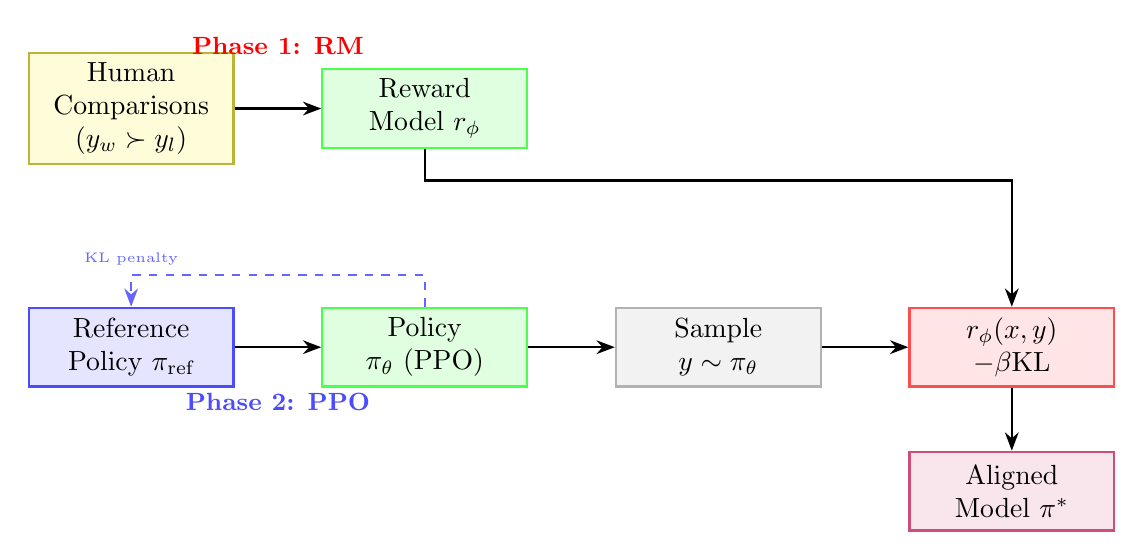
\begin{tikzpicture}[node distance=0.7cm and 1.1cm]
  % Phase 1: RM training
  \node[datblk] (human) {Human\\Comparisons\\$(y_w \succ y_l)$};
  \node[trnblk, right=of human] (rm) {Reward\\Model $r_\phi$};

  % Phase 2: PPO
  \node[frzblk, below=1.8cm of human] (ref) {Reference\\Policy $\pi_{\text{ref}}$};
  \node[trnblk, right=of ref] (policy) {Policy\\$\pi_\theta$ (PPO)};
  \node[grayblk, right=of policy] (sample) {Sample\\$y \sim \pi_\theta$};
  \node[lossblk, right=of sample] (rloss) {$r_\phi(x,y)$\\$-\beta$KL};
  \node[mrgblk, below=0.8cm of rloss] (aligned) {Aligned\\Model $\pi^*$};

  \draw[arr] (human)--(rm);
  \draw[arr] (rm.south) -- ++(0,-0.4) -| (rloss.north);
  \draw[arr] (ref)--(policy);
  \draw[arr] (policy)--(sample);
  \draw[arr] (sample)--(rloss);
  \draw[arr] (rloss)--(aligned);
  \draw[arr,dashed,blue!60] (policy.north) -- ++(0,0.4) -| (ref.north) node[midway,above,font=\tiny]{KL penalty};

  \node[font=\small\bfseries,red] at ($(human)!0.5!(rm)+(0,0.8)$) {Phase 1: RM};
  \node[font=\small\bfseries,blue!70] at ($(ref)!0.5!(policy)+(0,-0.7)$) {Phase 2: PPO};
\end{tikzpicture}
\caption{RLHF: reward model trained on human comparisons then used to guide PPO policy optimisation.}
\end{figure}

\subsection{State Transition Table}
\begin{table}[h]\centering
\begin{tabular}{lll}\toprule
\textbf{Property} & \textbf{Before} & \textbf{After}\\\midrule
Policy type & SFT checkpoint & RLHF-aligned policy\\
Reward signal & None & Human preference score\\
KL from reference & 0 & Bounded by $\beta$\\
Human preference win-rate & $\sim$50\% & $>70$\%\\
Training complexity & Single loop & Two-phase (RM + PPO)\\\bottomrule
\end{tabular}
\caption{State properties before and after RLHF.}
\end{table}

\newpage
%% ------------------------------------------------------------
\section{Direct Preference Optimization (DPO)}

\subsection{Mathematical Foundation}
DPO reformulates RLHF into a single supervised objective, bypassing the explicit reward model. Starting from the closed-form optimal policy under KL constraint, the loss becomes:
\begin{equation}
  \mathcal{L}_{\text{DPO}} = -\mathbb{E}\!\left[\log\sigma\!\left(\beta\log\frac{\pi_\theta(y_w|x)}{\pi_{\text{ref}}(y_w|x)} - \beta\log\frac{\pi_\theta(y_l|x)}{\pi_{\text{ref}}(y_l|x)}\right)\right]
\end{equation}
The implicit reward is $r(x,y) = \beta\log(\pi_\theta(y|x)/\pi_{\text{ref}}(y|x))$. No sampling loop or value network is needed.

\subsection{Architecture Flow Diagram}

\begin{figure}[h]
\centering
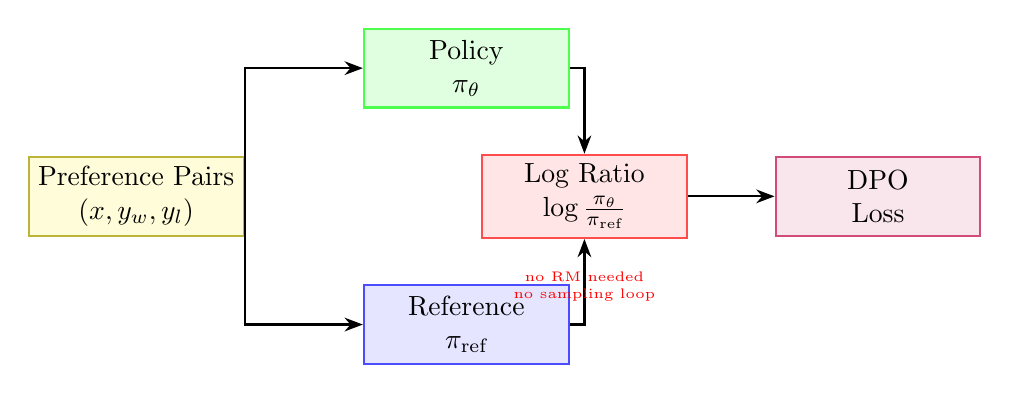
\begin{tikzpicture}[node distance=0.7cm and 1.1cm]
  \node[datblk] (pairs) {Preference Pairs\\$(x, y_w, y_l)$};
  \node[trnblk, above right=0.6cm and 1.5cm of pairs] (pol) {Policy\\$\pi_\theta$};
  \node[frzblk, below right=0.6cm and 1.5cm of pairs] (ref) {Reference\\$\pi_{\text{ref}}$};
  \node[lossblk, right=3.0cm of pairs] (ratio) {Log Ratio\\$\log\frac{\pi_\theta}{\pi_{\text{ref}}}$};
  \node[mrgblk, right=of ratio] (out) {DPO\\Loss};

  \draw[arr] (pairs.east) |- (pol.west);
  \draw[arr] (pairs.east) |- (ref.west);
  \draw[arr] (pol.east) -| (ratio.north);
  \draw[arr] (ref.east) -| (ratio.south);
  \draw[arr] (ratio)--(out);

  \node[font=\tiny,red,align=center,below=0.3cm of ratio] {no RM needed\\no sampling loop};
\end{tikzpicture}
\caption{DPO: both policy and frozen reference score chosen/rejected responses; loss uses their log-ratio difference.}
\end{figure}

\subsection{State Transition Table}
\begin{table}[h]\centering
\begin{tabular}{lll}\toprule
\textbf{Property} & \textbf{Before (RLHF)} & \textbf{After (DPO)}\\\midrule
Reward model & Explicit $r_\phi$ & Implicit in log-ratio\\
Sampling loop & Yes (PPO rollouts) & No\\
Reference policy & Frozen copy & Frozen copy\\
Training stability & Sensitive to reward hacking & More stable\\
Compute cost & High (2-phase) & Lower (single SFT-like pass)\\\bottomrule
\end{tabular}
\caption{State properties comparing RLHF and DPO.}
\end{table}

\newpage
%% ------------------------------------------------------------
\section{Identity Preference Optimization (IPO)}

\subsection{Mathematical Foundation}
IPO fixes a theoretical limitation of DPO: when the optimal policy places all mass on $y_w$, the DPO log-ratio diverges. IPO introduces a bounded objective by replacing the log-sigmoid with a squared-error hinge on the preference gap $h$:
\begin{equation}
  h(x,y_w,y_l) = \log\frac{\pi_\theta(y_w|x)}{\pi_{\text{ref}}(y_w|x)} - \log\frac{\pi_\theta(y_l|x)}{\pi_{\text{ref}}(y_l|x)}
\end{equation}
\begin{equation}
  \mathcal{L}_{\text{IPO}} = \mathbb{E}\!\left[\left(h(x,y_w,y_l) - \frac{1}{2\beta}\right)^2\right]
\end{equation}
The target $\frac{1}{2\beta}$ acts as a regulariser preventing the preference gap from growing unboundedly.

\subsection{Architecture Flow Diagram}

\begin{figure}[h]
\centering
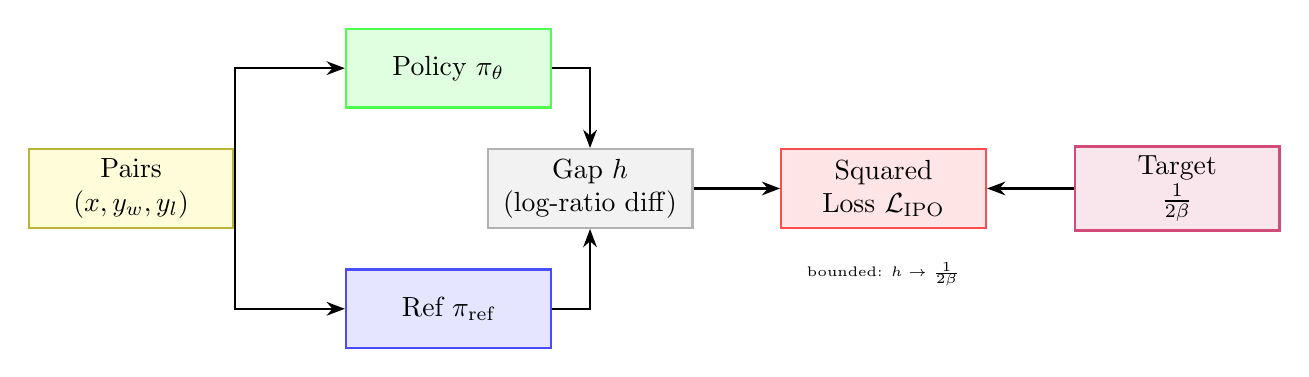
\begin{tikzpicture}[node distance=0.7cm and 1.1cm]
  \node[datblk] (pairs) {Pairs\\$(x,y_w,y_l)$};
  \node[trnblk, above right=0.5cm and 1.4cm of pairs] (pol) {Policy $\pi_\theta$};
  \node[frzblk, below right=0.5cm and 1.4cm of pairs] (ref) {Ref $\pi_{\text{ref}}$};
  \node[grayblk, right=3.2cm of pairs] (h) {Gap $h$\\(log-ratio diff)};
  \node[lossblk, right=of h] (loss) {Squared\\Loss $\mathcal{L}_{\text{IPO}}$};
  \node[mrgblk, right=of loss] (tgt) {Target\\$\frac{1}{2\beta}$};

  \draw[arr] (pairs.east)|-  (pol.west);
  \draw[arr] (pairs.east)|-  (ref.west);
  \draw[arr] (pol.east) -| (h.north);
  \draw[arr] (ref.east) -| (h.south);
  \draw[arr] (h)--(loss);
  \draw[arr] (tgt.west)--(loss.east);

  \node[font=\tiny,align=center,below=0.3cm of loss] {bounded: $h \to \frac{1}{2\beta}$};
\end{tikzpicture}
\caption{IPO: like DPO but the log-ratio gap is penalised toward a finite target $1/(2\beta)$.}
\end{figure}

\subsection{State Transition Table}
\begin{table}[h]\centering
\begin{tabular}{lll}\toprule
\textbf{Property} & \textbf{Before (DPO)} & \textbf{After (IPO)}\\\midrule
Loss type & Log-sigmoid & Squared error\\
Divergence at optimum & Unbounded & Bounded by $\frac{1}{2\beta}$\\
Target preference gap & Maximise & Converge to $\frac{1}{2\beta}$\\
Regularisation & KL implicit & Explicit squared bound\\
Training saturation & Can saturate & More stable\\\bottomrule
\end{tabular}
\caption{State properties comparing DPO and IPO.}
\end{table}

\newpage
%% ------------------------------------------------------------
\section{Odds Ratio Preference Optimization (ORPO)}

\subsection{Mathematical Foundation}
ORPO combines SFT loss and an odds-ratio contrast in a single objective — no reference model needed. The odds of generating $y$ under policy $\pi_\theta$ is $\text{odds}(y|x) = \pi_\theta(y|x)/(1-\pi_\theta(y|x))$. The combined loss is:
\begin{equation}
  \mathcal{L}_{\text{ORPO}} = \mathcal{L}_{\text{SFT}} - \lambda\,\mathbb{E}\!\left[\log\sigma\!\left(\log\frac{\text{odds}(y_w|x)}{\text{odds}(y_l|x)}\right)\right]
\end{equation}
The SFT term increases $\pi_\theta(y_w|x)$ while the odds-ratio term simultaneously penalises $y_l$ without requiring a frozen reference copy.

\subsection{Architecture Flow Diagram}

\begin{figure}[h]
\centering
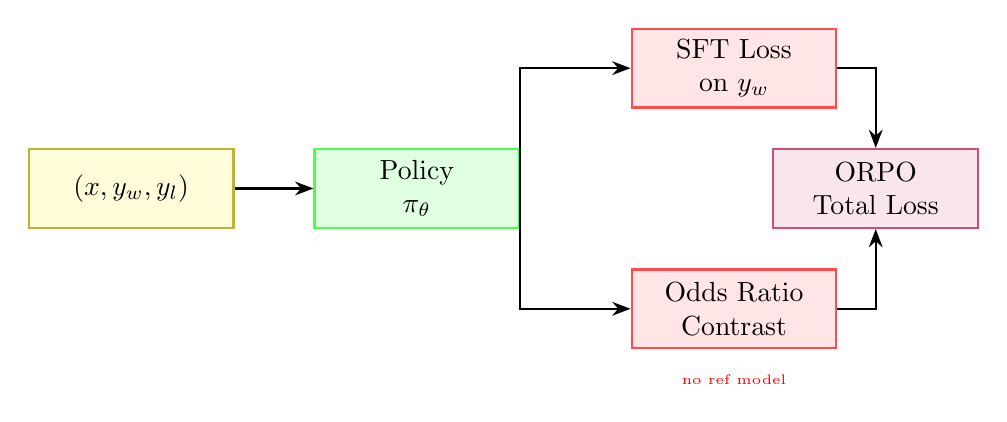
\begin{tikzpicture}[node distance=0.7cm and 1.0cm]
  \node[datblk] (data) {$(x, y_w, y_l)$};
  \node[trnblk, right=of data] (pol) {Policy\\$\pi_\theta$};
  \node[lossblk, above right=0.5cm and 1.4cm of pol] (sft) {SFT Loss\\on $y_w$};
  \node[lossblk, below right=0.5cm and 1.4cm of pol] (or) {Odds Ratio\\Contrast};
  \node[mrgblk, right=3.2cm of pol] (total) {ORPO\\Total Loss};

  \draw[arr] (data)--(pol);
  \draw[arr] (pol.east) |- (sft.west);
  \draw[arr] (pol.east) |- (or.west);
  \draw[arr] (sft.east) -| (total.north);
  \draw[arr] (or.east) -| (total.south);

  \node[font=\tiny,red,align=center,below=0.2cm of or] {no ref model};
\end{tikzpicture}
\caption{ORPO: SFT loss on the chosen response combined with an odds-ratio preference contrast.}
\end{figure}

\subsection{State Transition Table}
\begin{table}[h]\centering
\begin{tabular}{lll}\toprule
\textbf{Property} & \textbf{Before} & \textbf{After}\\\midrule
Reference model & Required (DPO/RLHF) & Not required\\
Training phases & 2 (SFT then align) & 1 (joint)\\
Loss terms & Single & SFT + odds-ratio\\
Memory overhead & $2\times$ model & $1\times$ model only\\
Data format & Prompt + completion & Triplet $(x, y_w, y_l)$\\\bottomrule
\end{tabular}
\caption{State properties before and after ORPO.}
\end{table}

\newpage
%% ------------------------------------------------------------
\section{Kahneman-Tversky Optimization (KTO)}

\subsection{Mathematical Foundation}
KTO aligns LLMs by maximising a utility function inspired by Kahneman-Tversky prospect theory. It operates on \emph{individual} samples labelled good ($z=1$) or bad ($z=0$), not pairwise comparisons:
\begin{equation}
  v(y, z) = \begin{cases} w_+(r(x,y) - r_{\text{KL}}) & z = 1 \\ w_-(r(x,y) - r_{\text{KL}}) & z = 0 \end{cases}
\end{equation}
\begin{equation}
  \mathcal{L}_{\text{KTO}} = \mathbb{E}\bigl[1 - v(y, z)\bigr]
\end{equation}
where $r_{\text{KL}} = \beta\,\text{KL}[\pi_\theta \| \pi_{\text{ref}}]$ is a KL-penalty baseline. The asymmetric weights $w_+ \neq w_-$ model loss-aversion.

\subsection{Architecture Flow Diagram}

\begin{figure}[h]
\centering
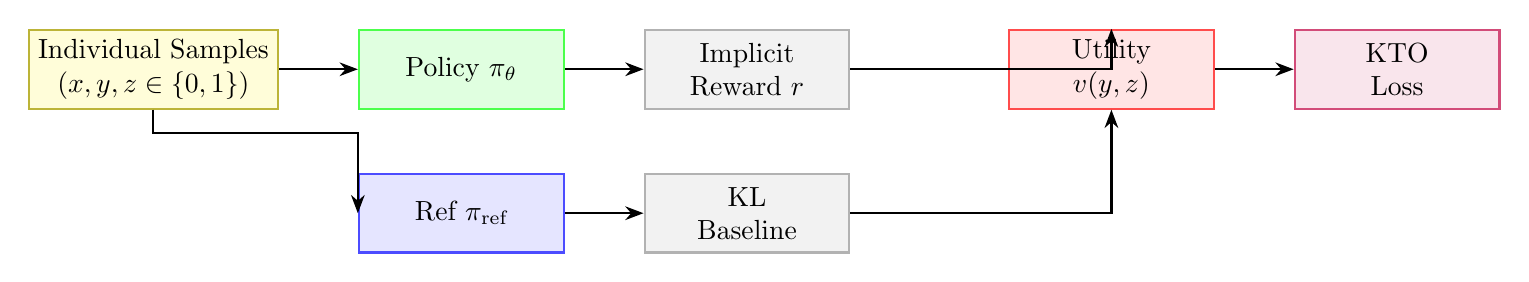
\begin{tikzpicture}[node distance=0.7cm and 1.0cm]
  \node[datblk] (data) {Individual Samples\\$(x, y, z\in\{0,1\})$};
  \node[trnblk, right=of data] (pol) {Policy $\pi_\theta$};
  \node[frzblk, below=0.8cm of pol] (ref) {Ref $\pi_{\text{ref}}$};
  \node[grayblk, right=of pol] (r) {Implicit\\Reward $r$};
  \node[grayblk, right=of ref] (kl) {KL\\Baseline};
  \node[lossblk, right=2.0cm of r] (util) {Utility\\$v(y,z)$};
  \node[mrgblk, right=of util] (out) {KTO\\Loss};

  \draw[arr] (data)--(pol);
  \draw[arr] (data.south) -- ++(0,-0.3) -| (ref.west);
  \draw[arr] (pol)--(r);
  \draw[arr] (ref)--(kl);
  \draw[arr] (r.east) -| (util.north);
  \draw[arr] (kl.east) -| (util.south);
  \draw[arr] (util)--(out);
\end{tikzpicture}
\caption{KTO: each sample is individually labelled good/bad; utility function uses prospect theory asymmetry.}
\end{figure}

\subsection{State Transition Table}
\begin{table}[h]\centering
\begin{tabular}{lll}\toprule
\textbf{Property} & \textbf{Before} & \textbf{After}\\\midrule
Data format & Pairwise $(y_w, y_l)$ & Individual $(y, z)$\\
Data collection effort & High (pairwise) & Lower (binary label)\\
Loss-aversion modelling & None & Asymmetric $w_+, w_-$\\
Reference model & Optional & Used for KL baseline\\
Applicable at scale & Full pairs required & Works with any ratio\\\bottomrule
\end{tabular}
\caption{State properties before and after KTO.}
\end{table}

\newpage
%% ------------------------------------------------------------
\section{Simple Preference Optimization (SimPO)}

\subsection{Mathematical Foundation}
SimPO eliminates the reference model by using average log-probability as an implicit reward and adding a target reward margin $\gamma$:
\begin{equation}
  r_{\text{SimPO}}(x,y) = \frac{\beta}{|y|}\log\pi_\theta(y \mid x)
\end{equation}
\begin{equation}
  \mathcal{L}_{\text{SimPO}} = -\mathbb{E}\!\left[\log\sigma\!\left(r_{\text{SimPO}}(x,y_w) - r_{\text{SimPO}}(x,y_l) - \gamma\right)\right]
\end{equation}
Length normalisation prevents the model from favouring short responses, and $\gamma > 0$ enforces a minimum gap between chosen and rejected rewards.

\subsection{Architecture Flow Diagram}

\begin{figure}[h]
\centering
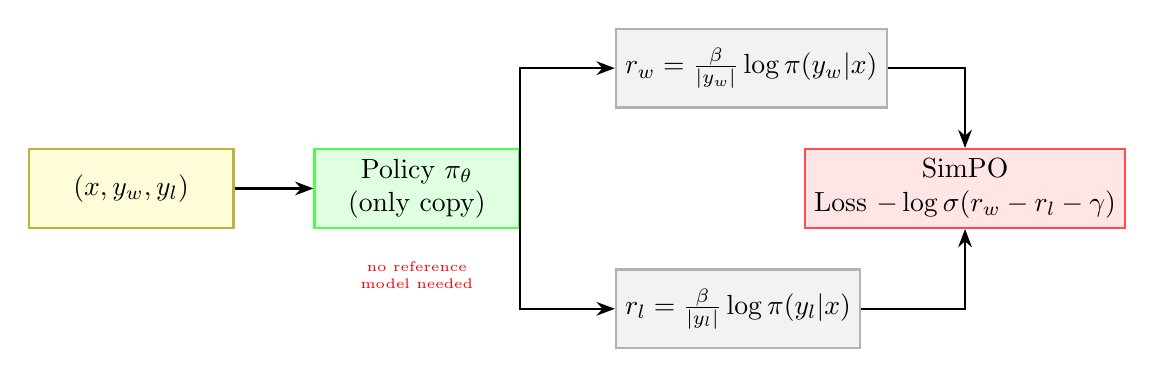
\begin{tikzpicture}[node distance=0.7cm and 1.0cm]
  \node[datblk] (data) {$(x, y_w, y_l)$};
  \node[trnblk, right=of data] (pol) {Policy $\pi_\theta$\\(only copy)};
  \node[grayblk, above right=0.5cm and 1.2cm of pol] (rw) {$r_w = \frac{\beta}{|y_w|}\log\pi(y_w|x)$};
  \node[grayblk, below right=0.5cm and 1.2cm of pol] (rl) {$r_l = \frac{\beta}{|y_l|}\log\pi(y_l|x)$};
  \node[lossblk, right=3.6cm of pol] (loss) {SimPO\\Loss $-\log\sigma(r_w - r_l - \gamma)$};

  \draw[arr] (data)--(pol);
  \draw[arr] (pol.east) |- (rw.west);
  \draw[arr] (pol.east) |- (rl.west);
  \draw[arr] (rw.east) -| (loss.north);
  \draw[arr] (rl.east) -| (loss.south);

  \node[red,font=\tiny,align=center,below=0.3cm of pol] {no reference\\model needed};
\end{tikzpicture}
\caption{SimPO: length-normalised log-probs replace the reference log-ratio; margin $\gamma$ enforces quality gap.}
\end{figure}

\subsection{State Transition Table}
\begin{table}[h]\centering
\begin{tabular}{lll}\toprule
\textbf{Property} & \textbf{Before (DPO)} & \textbf{After (SimPO)}\\\midrule
Reference model & Required & Not needed\\
Reward definition & Log-ratio $\pi/\pi_{\text{ref}}$ & Length-norm avg log-prob\\
Length bias & Possible & Mitigated by $1/|y|$\\
Margin hyperparameter & None & $\gamma > 0$\\
Memory saving & None & No second model forward pass\\\bottomrule
\end{tabular}
\caption{State properties comparing DPO and SimPO.}
\end{table}

\newpage
%% ------------------------------------------------------------
\section{Constrained Preference Optimization (CPO)}

\subsection{Mathematical Foundation}
CPO formulates alignment as a constrained optimisation: maximise reward while staying within a trust region $\epsilon$ of the reference policy measured in reverse KL divergence:
\begin{equation}
  \max_{\pi_\theta} \mathbb{E}[r(x,y)] \quad \text{s.t.} \quad \mathbb{KL}[\pi_{\text{ref}} \| \pi_\theta] \leq \epsilon
\end{equation}
The Lagrangian relaxation yields a combined training objective:
\begin{equation}
  \mathcal{L}_{\text{CPO}} = -\mathbb{E}[r(x,y)] + \mu\bigl(\mathbb{KL}[\pi_{\text{ref}} \| \pi_\theta] - \epsilon\bigr)
\end{equation}
where $\mu \geq 0$ is a dual variable updated online to enforce the constraint.

\subsection{Architecture Flow Diagram}

\begin{figure}[h]
\centering
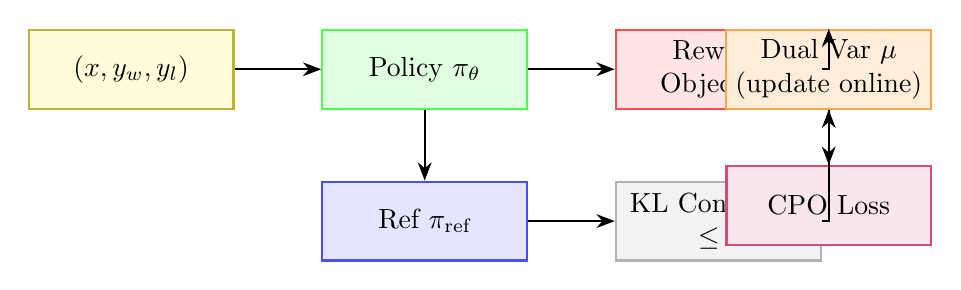
\begin{tikzpicture}[node distance=0.7cm and 1.1cm]
  \node[datblk] (data) {$(x, y_w, y_l)$};
  \node[trnblk, right=of data] (pol) {Policy $\pi_\theta$};
  \node[frzblk, below=0.9cm of pol] (ref) {Ref $\pi_{\text{ref}}$};
  \node[lossblk, right=of pol] (rew) {Reward\\Objective};
  \node[grayblk, right=of ref] (kl) {KL Constraint\\$\leq \epsilon$};
  \node[orangeblk, right=2.5cm of pol] (mu) {Dual Var $\mu$\\(update online)};
  \node[mrgblk, below=0.7cm of mu] (out) {CPO Loss};

  \draw[arr] (data)--(pol);
  \draw[arr] (pol)--(rew);
  \draw[arr] (pol.south)--(ref.north);
  \draw[arr] (ref)--(kl);
  \draw[arr] (rew.east)-|(mu.north);
  \draw[arr] (kl.east)-|(mu.south);
  \draw[arr] (mu)--(out);
\end{tikzpicture}
\caption{CPO: reward maximisation with an explicit KL constraint; dual variable $\mu$ adapts online.}
\end{figure}

\subsection{State Transition Table}
\begin{table}[h]\centering
\begin{tabular}{lll}\toprule
\textbf{Property} & \textbf{Before} & \textbf{After}\\\midrule
Constraint form & Soft KL penalty & Hard KL constraint $\leq \epsilon$\\
Dual variable $\mu$ & Fixed & Dynamically updated\\
Policy deviation & Unbounded & Bounded within trust region\\
Reward maximisation & Soft & Subject to constraint\\
Training dynamics & Standard & Saddle-point optimisation\\\bottomrule
\end{tabular}
\caption{State properties before and after CPO.}
\end{table}

\newpage
%% ------------------------------------------------------------
\section{Anchored Preference Optimization (APO)}

\subsection{Mathematical Foundation}
APO introduces an anchor term that explicitly regularises the policy toward the reference model while simultaneously pushing chosen responses up and rejected responses down:
\begin{equation}
  \mathcal{L}_{\text{APO}} = \mathbb{E}\!\left[\underbrace{-\log\sigma\bigl(\beta(r_w - r_l)\bigr)}_{\text{preference}} + \lambda\underbrace{\bigl(\log\frac{\pi_\theta(y_w|x)}{\pi_{\text{ref}}(y_w|x)} - \log\frac{\pi_\theta(y_l|x)}{\pi_{\text{ref}}(y_l|x)}\bigr)^2}_{\text{anchor}}\right]
\end{equation}
The anchor term is minimised when both the chosen and rejected log-ratios equal a fixed reference, preventing the model from drifting.

\subsection{Architecture Flow Diagram}

\begin{figure}[h]
\centering
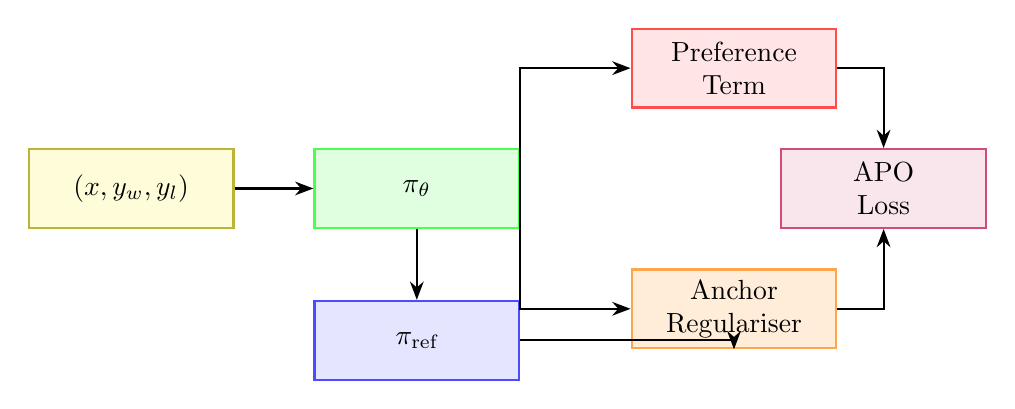
\begin{tikzpicture}[node distance=0.7cm and 1.0cm]
  \node[datblk] (data) {$(x,y_w,y_l)$};
  \node[trnblk, right=of data] (pol) {$\pi_\theta$};
  \node[frzblk, below=0.9cm of pol] (ref) {$\pi_{\text{ref}}$};
  \node[lossblk, above right=0.5cm and 1.4cm of pol] (pref) {Preference\\Term};
  \node[orangeblk, below right=0.5cm and 1.4cm of pol] (anchor) {Anchor\\Regulariser};
  \node[mrgblk, right=3.3cm of pol] (total) {APO\\Loss};

  \draw[arr] (data)--(pol);
  \draw[arr] (pol.east) |- (pref.west);
  \draw[arr] (pol.south)--(ref.north);
  \draw[arr] (ref.east) -| (anchor.south);
  \draw[arr] (pol.east) |- (anchor.west);
  \draw[arr] (pref.east) -| (total.north);
  \draw[arr] (anchor.east) -| (total.south);
\end{tikzpicture}
\caption{APO: combines standard preference loss with an anchor regulariser against the reference model.}
\end{figure}

\subsection{State Transition Table}
\begin{table}[h]\centering
\begin{tabular}{lll}\toprule
\textbf{Property} & \textbf{Before (DPO)} & \textbf{After (APO)}\\\midrule
Anchor regularisation & Implicit KL & Explicit squared anchor\\
Reference role & Log-ratio denominator & Explicit target\\
Policy drift & Can drift & Penalised\\
Loss terms & 1 & 2 (preference + anchor)\\
Stability & Moderate & Higher (dual grounding)\\\bottomrule
\end{tabular}
\caption{State properties comparing DPO and APO.}
\end{table}

\newpage
%% ------------------------------------------------------------
\section{Rank Responses from Human Feedback (RRHF)}

\subsection{Mathematical Foundation}
RRHF generates $K$ candidate responses $\{y^{(1)}, \ldots, y^{(K)}\}$ from the model, ranks them by human or AI annotators, and trains the model to assign higher log-probability to higher-ranked responses via a pairwise ranking loss:
\begin{equation}
  \mathcal{L}_{\text{RRHF}} = \sum_{i < j}\max\!\bigl(0,\, \text{score}(y^{(j)}) - \text{score}(y^{(i)}) + \delta\bigr) + \lambda \mathcal{L}_{\text{SFT}}(y^{(1)})
\end{equation}
where $\text{score}(y^{(k)}) = \log P_\theta(y^{(k)}|x)/|y^{(k)}|$ is the normalised log-prob. The SFT term anchors the top-ranked response.

\subsection{Architecture Flow Diagram}

\begin{figure}[h]
\centering
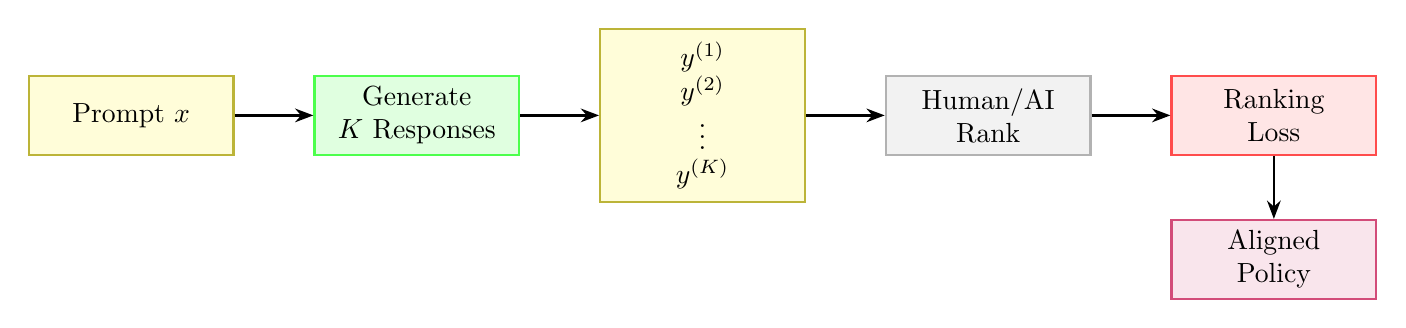
\begin{tikzpicture}[node distance=0.6cm and 1.0cm]
  \node[datblk] (x) {Prompt $x$};
  \node[trnblk, right=of x] (gen) {Generate\\$K$ Responses};
  \node[datblk, right=of gen, minimum height=2.2cm] (cands) {$y^{(1)}$\\$y^{(2)}$\\$\vdots$\\$y^{(K)}$};
  \node[grayblk, right=of cands] (rank) {Human/AI\\Rank};
  \node[lossblk, right=of rank] (loss) {Ranking\\Loss};
  \node[mrgblk, below=0.8cm of loss] (out) {Aligned\\Policy};

  \draw[arr] (x)--(gen);
  \draw[arr] (gen)--(cands);
  \draw[arr] (cands)--(rank);
  \draw[arr] (rank)--(loss);
  \draw[arr] (loss)--(out);
\end{tikzpicture}
\caption{RRHF: $K$ responses are generated and ranked; policy trained to match rank order via pairwise loss.}
\end{figure}

\subsection{State Transition Table}
\begin{table}[h]\centering
\begin{tabular}{lll}\toprule
\textbf{Property} & \textbf{Before} & \textbf{After}\\\midrule
Responses per prompt & 1 & $K$ (ranked)\\
Supervision signal & Binary (win/lose) & Full rank ordering\\
Loss type & Log-sigmoid & Pairwise margin\\
Top-response training & Separate SFT & Joint SFT + ranking\\
Annotation granularity & Single comparison & Full $K$-way ranking\\\bottomrule
\end{tabular}
\caption{State properties before and after RRHF.}
\end{table}

\newpage
%% ------------------------------------------------------------
\section{Reinforcement Learning from AI Feedback (RLAIF)}

\subsection{Mathematical Foundation}
RLAIF replaces expensive human annotators with a capable AI model (``AI annotator'' $\mathcal{A}$) to generate preference labels at scale. The AI annotator scores pairs via a prompt $p$:
\begin{equation}
  \hat{r}(x,y_i,y_j) = P_\mathcal{A}(y_i \succ y_j \mid p,\, x,\, y_i,\, y_j)
\end{equation}
These AI-generated preferences are then used identically to human preferences to train the RM and run PPO (or DPO):
\begin{equation}
  \mathcal{L}_{\text{RLAIF}} = -\mathbb{E}\!\left[\log\sigma\!\left(r_\phi(x,y_w) - r_\phi(x,y_l)\right)\right], \quad (y_w \succ y_l) \text{ from } \mathcal{A}
\end{equation}

\subsection{Architecture Flow Diagram}

\begin{figure}[h]
\centering
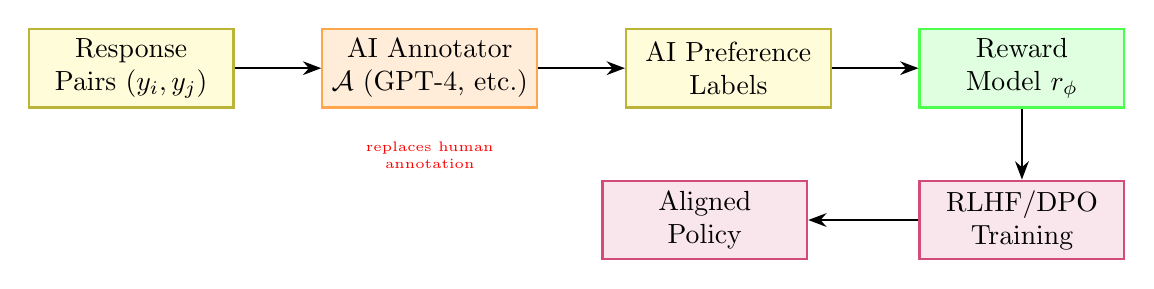
\begin{tikzpicture}[node distance=0.7cm and 1.1cm]
  \node[datblk] (pairs) {Response\\Pairs $(y_i, y_j)$};
  \node[orangeblk, right=of pairs] (ai) {AI Annotator\\$\mathcal{A}$ (GPT-4, etc.)};
  \node[datblk, right=of ai] (prefs) {AI Preference\\Labels};
  \node[trnblk, right=of prefs] (rm) {Reward\\Model $r_\phi$};
  \node[mrgblk, below=0.9cm of rm] (ppo) {RLHF/DPO\\Training};
  \node[mrgblk, left=1.4cm of ppo] (out) {Aligned\\Policy};

  \draw[arr] (pairs)--(ai);
  \draw[arr] (ai)--(prefs);
  \draw[arr] (prefs)--(rm);
  \draw[arr] (rm)--(ppo);
  \draw[arr] (ppo)--(out);

  \node[font=\tiny,red,align=center,below=0.3cm of ai] {replaces human\\annotation};
\end{tikzpicture}
\caption{RLAIF: an AI model generates preference labels at scale, replacing costly human annotators.}
\end{figure}

\subsection{State Transition Table}
\begin{table}[h]\centering
\begin{tabular}{lll}\toprule
\textbf{Property} & \textbf{Before (RLHF)} & \textbf{After (RLAIF)}\\\midrule
Annotation source & Humans & AI annotator $\mathcal{A}$\\
Annotation cost & High (\$\$\$) & Low (API calls)\\
Annotation scale & Limited (thousands) & Massive (millions)\\
Annotation consistency & Variable & Consistent per model\\
Annotation bias & Human bias & AI model bias\\\bottomrule
\end{tabular}
\caption{State properties comparing RLHF and RLAIF.}
\end{table}

\newpage
%% ------------------------------------------------------------
\section{Constitutional AI}

\subsection{Mathematical Foundation}
Constitutional AI uses a set of principles $\mathcal{C} = \{c_1, \ldots, c_M\}$ (the ``constitution'') to iteratively critique and revise model outputs before training. In the RL phase, an AI Feedback model scores responses against the constitution:
\begin{equation}
  r_{\text{CAI}}(x, y) = \frac{1}{M}\sum_{m=1}^{M} P_\mathcal{A}(\text{harmless} \mid c_m, x, y)
\end{equation}
Two training phases: (1) supervised revision via critique-revise loop, (2) RLHF with AI-generated preference labels from the constitution.

\subsection{Architecture Flow Diagram}

\begin{figure}[h]
\centering
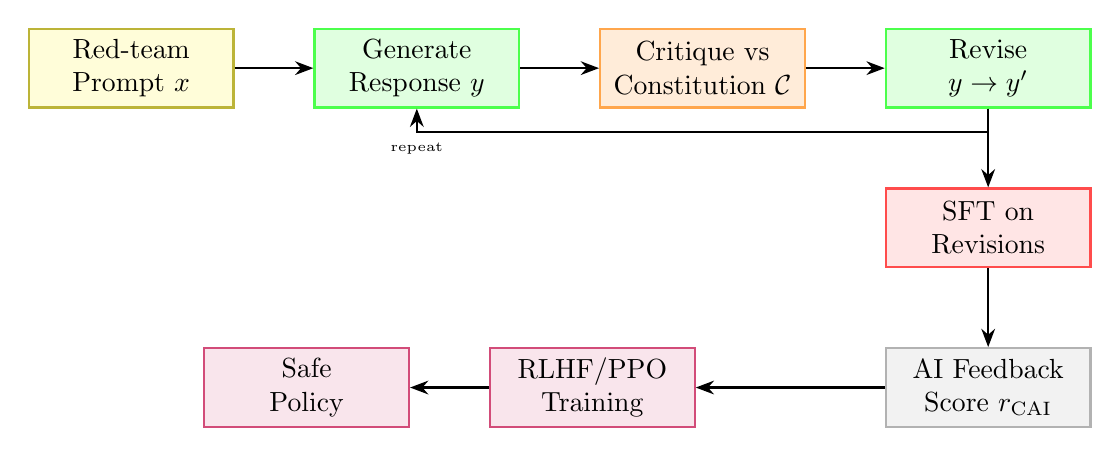
\begin{tikzpicture}[node distance=0.65cm and 1.0cm]
  % Critique-revise loop
  \node[datblk] (red) {Red-team\\Prompt $x$};
  \node[trnblk, right=of red] (gen) {Generate\\Response $y$};
  \node[orangeblk, right=of gen] (crit) {Critique vs\\Constitution $\mathcal{C}$};
  \node[trnblk, right=of crit] (rev) {Revise\\$y \to y'$};

  % SFT on revisions
  \node[lossblk, below=1.0cm of rev] (sft) {SFT on\\Revisions};

  % RL phase
  \node[grayblk, below=1.0cm of sft] (aifb) {AI Feedback\\Score $r_{\text{CAI}}$};
  \node[mrgblk, left=2.4cm of aifb] (rl) {RLHF/PPO\\Training};
  \node[mrgblk, left=of rl] (out) {Safe\\Policy};

  \draw[arr] (red)--(gen);
  \draw[arr] (gen)--(crit);
  \draw[arr] (crit)--(rev);
  \draw[arr] (rev.south) -- ++(0,-0.3) -| (gen.south) node[midway,below,font=\tiny]{repeat};
  \draw[arr] (rev)--(sft);
  \draw[arr] (sft)--(aifb);
  \draw[arr] (aifb)--(rl);
  \draw[arr] (rl)--(out);
\end{tikzpicture}
\caption{Constitutional AI: critique-revise loop creates SFT data; AI feedback from constitution guides RLHF.}
\end{figure}

\subsection{State Transition Table}
\begin{table}[h]\centering
\begin{tabular}{lll}\toprule
\textbf{Property} & \textbf{Before} & \textbf{After}\\\midrule
Safety signal & None / Human labels & AI + constitutionl principles\\
Training phases & SFT only & Critique-revise SFT + RLAIF\\
Red-team coverage & Manual & Systematic via constitution\\
Harmlessness & Moderate & Substantially improved\\
Helpfulness trade-off & N/A & Explicitly balanced\\\bottomrule
\end{tabular}
\caption{State properties before and after Constitutional AI training.}
\end{table}

\newpage
%% ============================================================
\part{Reinforcement Learning Training Methods}
%% ============================================================

\section{Proximal Policy Optimization (PPO)}

\subsection{Mathematical Foundation}
PPO is the core RL algorithm used in RLHF. It clips the probability ratio to prevent large policy updates:
\begin{equation}
  \rho_t = \frac{\pi_\theta(a_t|s_t)}{\pi_{\theta_{\text{old}}}(a_t|s_t)},\quad \hat{A}_t = r_t + \gamma V(s_{t+1}) - V(s_t)
\end{equation}
\begin{equation}
  \mathcal{L}_{\text{PPO}} = -\mathbb{E}_t\bigl[\min\!\bigl(\rho_t \hat{A}_t,\; \text{clip}(\rho_t, 1-\epsilon, 1+\epsilon)\hat{A}_t\bigr)\bigr]
\end{equation}
A value network $V_\phi$ is trained simultaneously. For LLMs, tokens are actions and the RM score at end-of-sequence provides the sparse reward.

\subsection{Architecture Flow Diagram}

\begin{figure}[h]
\centering
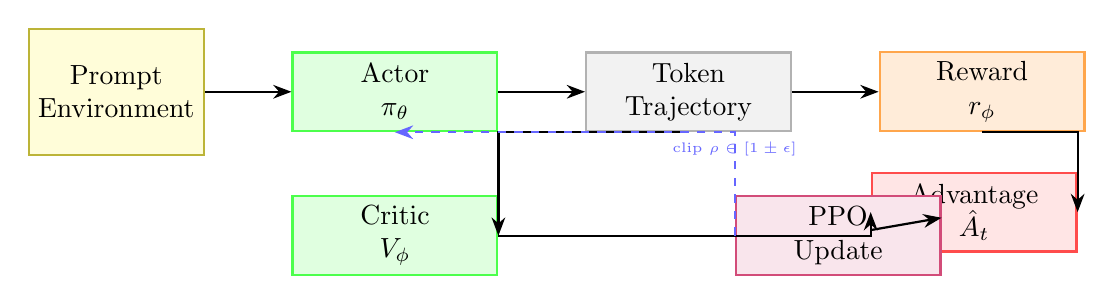
\begin{tikzpicture}[node distance=0.7cm and 1.1cm]
  \node[datblk, minimum size=1.6cm] (env) {Prompt\\Environment};
  \node[trnblk, right=of env] (actor) {Actor\\$\pi_\theta$};
  \node[trnblk, below=0.8cm of actor] (critic) {Critic\\$V_\phi$};
  \node[grayblk, right=of actor] (traj) {Token\\Trajectory};
  \node[orangeblk, right=of traj] (rm) {Reward\\$r_\phi$};
  \node[lossblk, below right=0.5cm and 1.0cm of traj] (adv) {Advantage\\$\hat{A}_t$};
  \node[mrgblk, right=3.0cm of critic] (upd) {PPO\\Update};

  \draw[arr] (env)--(actor);
  \draw[arr] (actor)--(traj);
  \draw[arr] (traj)--(rm);
  \draw[arr] (traj.south) -| (critic.east);
  \draw[arr] (rm.south) -| (adv.east);
  \draw[arr] (critic.east) -| (adv.west);
  \draw[arr] (adv)--(upd);
  \draw[arr,dashed,blue!60] (upd.west) |- (actor.south) node[midway,below,font=\tiny]{clip $\rho \in [1\pm\epsilon]$};
\end{tikzpicture}
\caption{PPO: actor generates trajectory, critic estimates value, advantage drives clipped surrogate update.}
\end{figure}

\subsection{State Transition Table}
\begin{table}[h]\centering
\begin{tabular}{lll}\toprule
\textbf{Property} & \textbf{Before} & \textbf{After}\\\midrule
Policy update size & Unconstrained & Clipped by $\epsilon$\\
Value network & None & Trained $V_\phi$\\
Advantage estimation & N/A & GAE $\hat{A}_t$\\
Training stability & Unstable (vanilla PG) & Stable (clip constraint)\\
Reward signal & Sparse (end of seq) & Discounted returns\\\bottomrule
\end{tabular}
\caption{State properties before and after PPO setup.}
\end{table}

\newpage
%% ------------------------------------------------------------
\section{Group Relative Policy Optimization (GRPO)}

\subsection{Mathematical Foundation}
GRPO removes the critic (value network) by using group-level reward statistics. For a prompt $x$, it samples $G$ outputs $\{y^{(1)},\ldots,y^{(G)}\}$ and computes relative advantages within the group:
\begin{equation}
  \hat{A}^{(i)} = \frac{r^{(i)} - \text{mean}(r^{(1:G)})}{\text{std}(r^{(1:G)})}
\end{equation}
\begin{equation}
  \mathcal{L}_{\text{GRPO}} = -\frac{1}{G}\sum_{i=1}^G \min\!\bigl(\rho^{(i)}\hat{A}^{(i)},\; \text{clip}(\rho^{(i)},1\pm\epsilon)\hat{A}^{(i)}\bigr) + \beta\,\text{KL}[\pi_\theta\|\pi_{\text{ref}}]
\end{equation}

\subsection{Architecture Flow Diagram}

\begin{figure}[h]
\centering
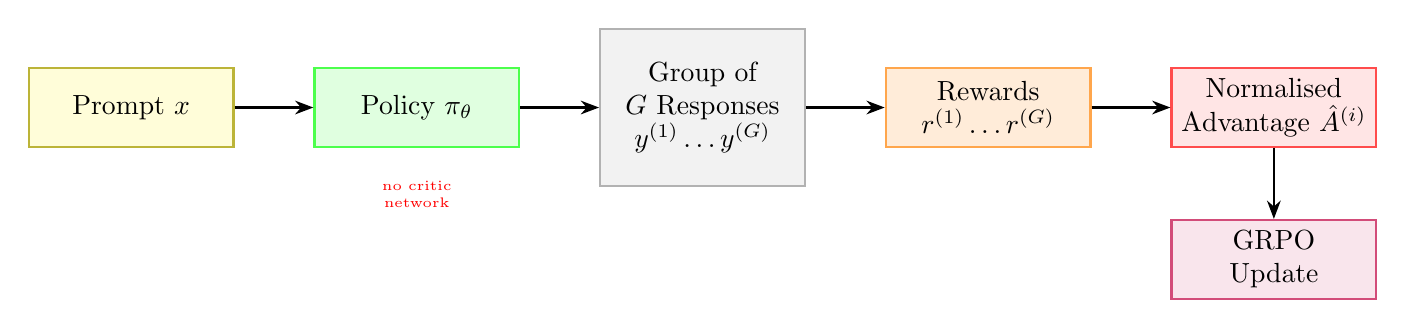
\begin{tikzpicture}[node distance=0.6cm and 1.0cm]
  \node[datblk] (x) {Prompt $x$};
  \node[trnblk, right=of x] (pol) {Policy $\pi_\theta$};
  \node[grayblk, right=of pol, minimum height=2.0cm] (group) {Group of\\$G$ Responses\\$y^{(1)}\ldots y^{(G)}$};
  \node[orangeblk, right=of group] (scores) {Rewards\\$r^{(1)}\ldots r^{(G)}$};
  \node[lossblk, right=of scores] (adv) {Normalised\\Advantage $\hat{A}^{(i)}$};
  \node[mrgblk, below=0.9cm of adv] (upd) {GRPO\\Update};

  \draw[arr] (x)--(pol);
  \draw[arr] (pol)--(group);
  \draw[arr] (group)--(scores);
  \draw[arr] (scores)--(adv);
  \draw[arr] (adv)--(upd);

  \node[red,font=\tiny,align=center,below=0.3cm of pol] {no critic\\network};
\end{tikzpicture}
\caption{GRPO: group of responses scored together; within-group normalised reward replaces value network.}
\end{figure}

\subsection{State Transition Table}
\begin{table}[h]\centering
\begin{tabular}{lll}\toprule
\textbf{Property} & \textbf{Before (PPO)} & \textbf{After (GRPO)}\\\midrule
Critic / value network & Required & Not needed\\
Advantage estimation & GAE (per token) & Group normalisation\\
Memory overhead & $2\times$ model (actor + critic) & $\approx 1\times$ model\\
Samples per prompt & 1 & $G$ (group sampling)\\
Variance reduction & Value baseline & Mean group reward\\\bottomrule
\end{tabular}
\caption{State properties comparing PPO and GRPO.}
\end{table}

\newpage
%% ------------------------------------------------------------
\section{Rejection Fine-Tuning (RFT)}

\subsection{Mathematical Foundation}
RFT generates $K$ candidate solutions per problem using the current policy, filters by a correctness verifier $\mathcal{V}$, and fine-tunes on the correct subset — essentially a self-improvement loop without RL:
\begin{equation}
  \mathcal{D}_{\text{correct}} = \{(x, y^{(k)}) : \mathcal{V}(x, y^{(k)}) = 1,\; y^{(k)} \sim \pi_\theta,\; k=1..K\}
\end{equation}
\begin{equation}
  \mathcal{L}_{\text{RFT}} = -\sum_{(x,y) \in \mathcal{D}_{\text{correct}}} \sum_t \log P_\theta(y_t \mid x, y_{<t})
\end{equation}
The process repeats: train on correct outputs, generate new candidates, filter again.

\subsection{Architecture Flow Diagram}

\begin{figure}[h]
\centering
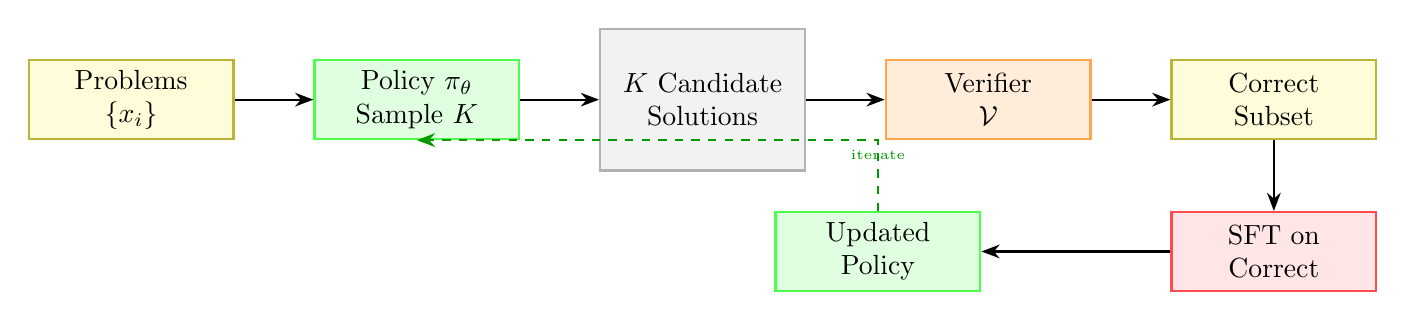
\begin{tikzpicture}[node distance=0.7cm and 1.0cm]
  \node[datblk] (prob) {Problems\\$\{x_i\}$};
  \node[trnblk, right=of prob] (pol) {Policy $\pi_\theta$\\Sample $K$};
  \node[grayblk, right=of pol, minimum height=1.8cm] (cands) {$K$ Candidate\\Solutions};
  \node[orangeblk, right=of cands] (ver) {Verifier\\$\mathcal{V}$};
  \node[datblk, right=of ver] (correct) {Correct\\Subset};
  \node[lossblk, below=0.9cm of correct] (sft) {SFT on\\Correct};
  \node[trnblk, left=2.4cm of sft] (newpol) {Updated\\Policy};

  \draw[arr] (prob)--(pol);
  \draw[arr] (pol)--(cands);
  \draw[arr] (cands)--(ver);
  \draw[arr] (ver)--(correct);
  \draw[arr] (correct)--(sft);
  \draw[arr] (sft)--(newpol);
  \draw[arr,dashed,green!60!black] (newpol.north) |- (pol.south) node[midway,below,font=\tiny]{iterate};
\end{tikzpicture}
\caption{RFT: policy samples $K$ solutions, verifier filters correct ones, SFT improves the policy iteratively.}
\end{figure}

\subsection{State Transition Table}
\begin{table}[h]\centering
\begin{tabular}{lll}\toprule
\textbf{Property} & \textbf{Before} & \textbf{After}\\\midrule
Data source & Static human labels & Self-generated correct solutions\\
RL component & Required (PPO) & None (SFT only)\\
Verifier & None & Required (exact-match, unit tests)\\
Pass@K improvement & Baseline & Improves with iterations\\
Training complexity & High (RL) & Standard SFT loop\\\bottomrule
\end{tabular}
\caption{State properties before and after RFT.}
\end{table}

\newpage
%% ------------------------------------------------------------
\section{REINFORCE}

\subsection{Mathematical Foundation}
REINFORCE is the foundational policy gradient algorithm. For a trajectory $\tau = (s_0,a_0,s_1,a_1,\ldots)$, the gradient of expected return is:
\begin{equation}
  \nabla_\theta J(\theta) = \mathbb{E}_{\tau \sim \pi_\theta}\!\left[G(\tau) \nabla_\theta \log \pi_\theta(\tau)\right],\quad G(\tau) = \sum_{t=0}^T \gamma^t r_t
\end{equation}
For LLMs, the trajectory is the token sequence, each token is an action, and $r_T$ (end reward) is discounted back. A baseline $b$ (e.g., mean reward) reduces variance:
\begin{equation}
  \nabla_\theta J \approx \frac{1}{N}\sum_n (G_n - b)\nabla_\theta \log \pi_\theta(y_n|x_n)
\end{equation}

\subsection{Architecture Flow Diagram}

\begin{figure}[h]
\centering
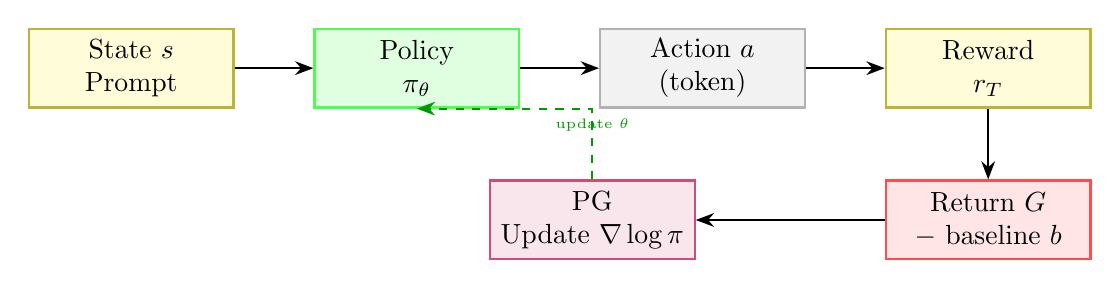
\begin{tikzpicture}[node distance=0.7cm and 1.0cm]
  \node[datblk] (state) {State $s$\\Prompt};
  \node[trnblk, right=of state] (pol) {Policy\\$\pi_\theta$};
  \node[grayblk, right=of pol] (act) {Action $a$\\(token)};
  \node[datblk, right=of act] (rew) {Reward\\$r_T$};
  \node[lossblk, below=0.9cm of rew] (ret) {Return $G$\\$-$ baseline $b$};
  \node[mrgblk, left=2.4cm of ret] (upd) {PG\\Update $\nabla\log\pi$};

  \draw[arr] (state)--(pol);
  \draw[arr] (pol)--(act);
  \draw[arr] (act)--(rew);
  \draw[arr] (rew)--(ret);
  \draw[arr] (ret)--(upd);
  \draw[arr,dashed,green!60!black] (upd.north) |- (pol.south) node[midway,below,font=\tiny]{update $\theta$};
\end{tikzpicture}
\caption{REINFORCE: policy samples action sequence, receives return $G$, updates via policy gradient.}
\end{figure}

\subsection{State Transition Table}
\begin{table}[h]\centering
\begin{tabular}{lll}\toprule
\textbf{Property} & \textbf{Before} & \textbf{After}\\\midrule
Gradient type & Supervised CE & Policy gradient $G\nabla\log\pi$\\
Variance & N/A & High (needs baseline)\\
Critic network & Not needed & Not needed\\
Reward type & N/A & Any differentiable or sparse\\
Update frequency & Per batch & Per episode/trajectory\\\bottomrule
\end{tabular}
\caption{State properties before and after REINFORCE setup.}
\end{table}

\newpage
%% ------------------------------------------------------------
\section{Advantage Actor-Critic (A2C / A3C)}

\subsection{Mathematical Foundation}
A2C uses a shared backbone with two heads: a policy head (actor) and a value head (critic). The advantage $A(s,a) = Q(s,a) - V(s)$ reduces gradient variance:
\begin{equation}
  \mathcal{L}_{\text{actor}} = -\mathbb{E}_t\bigl[A(s_t,a_t)\log\pi_\theta(a_t|s_t)\bigr]
\end{equation}
\begin{equation}
  \mathcal{L}_{\text{critic}} = \mathbb{E}_t\bigl[(r_t + \gamma V(s_{t+1}) - V(s_t))^2\bigr]
\end{equation}
A3C extends A2C with asynchronous parallel workers each running independent environments and gradients are asynchronously applied to a central parameter server.

\subsection{Architecture Flow Diagram}

\begin{figure}[h]
\centering
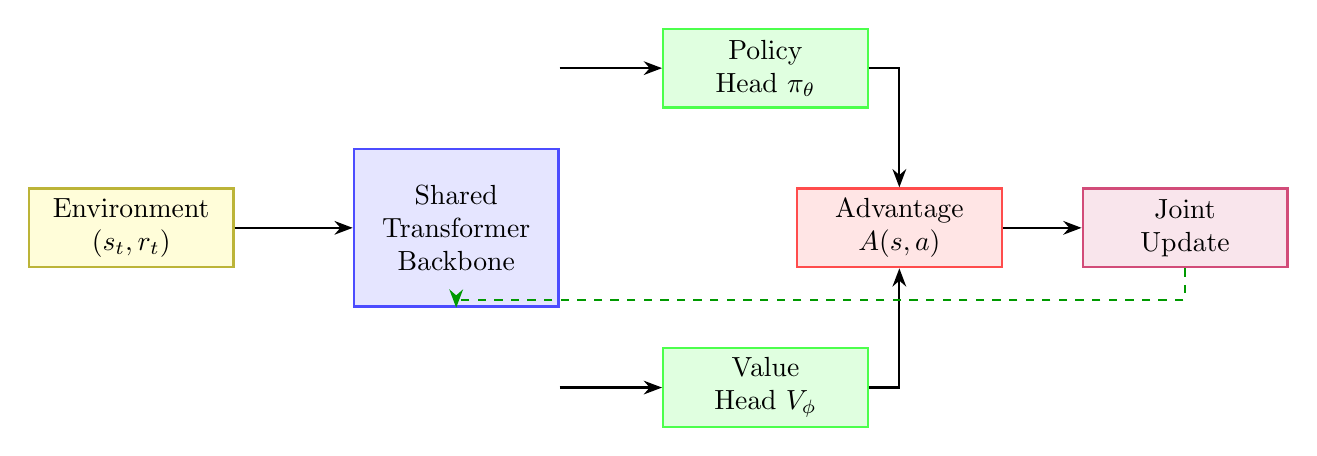
\begin{tikzpicture}[node distance=0.7cm and 1.0cm]
  \node[frzblk, minimum height=2.0cm] (backbone) {Shared\\Transformer\\Backbone};
  \node[trnblk, above right=0.5cm and 1.3cm of backbone] (actor) {Policy\\Head $\pi_\theta$};
  \node[trnblk, below right=0.5cm and 1.3cm of backbone] (critic) {Value\\Head $V_\phi$};
  \node[datblk, left=1.5cm of backbone] (env) {Environment\\$(s_t, r_t)$};
  \node[lossblk, right=3.0cm of backbone] (adv) {Advantage\\$A(s,a)$};
  \node[mrgblk, right=of adv] (upd) {Joint\\Update};

  \draw[arr] (env)--(backbone);
  \draw[arr] (backbone.east|-actor)--(actor.west);
  \draw[arr] (backbone.east|-critic)--(critic.west);
  \draw[arr] (actor.east) -| (adv.north);
  \draw[arr] (critic.east) -| (adv.south);
  \draw[arr] (adv)--(upd);
  \draw[arr,dashed,green!60!black] (upd.south) -- ++(0,-0.4) -| (backbone.south);
\end{tikzpicture}
\caption{A2C: shared backbone feeds actor (policy) and critic (value) heads; advantage combines their outputs.}
\end{figure}

\subsection{State Transition Table}
\begin{table}[h]\centering
\begin{tabular}{lll}\toprule
\textbf{Property} & \textbf{Before (REINFORCE)} & \textbf{After (A2C)}\\\midrule
Variance reduction & Baseline only & Full advantage estimation\\
Value network & Separate & Shared backbone, separate head\\
Gradient stability & Low & Higher (advantage)\\
Parallelism & None & A3C: asynchronous workers\\
Sample efficiency & Low & Higher (on-policy)\\\bottomrule
\end{tabular}
\caption{State properties comparing REINFORCE and A2C.}
\end{table}

\newpage
%% ------------------------------------------------------------
\section{Self-Play Reinforcement Learning}

\subsection{Mathematical Foundation}
In Self-Play RL, the model competes against previous versions of itself. At iteration $n$, the opponent is a snapshot $\pi_{\theta_{n-1}}$ (or mixture of past policies). The reward is determined by competitive outcome:
\begin{equation}
  r(y_{\theta}, y_{\theta_{\text{old}}}) = \begin{cases} +1 & \text{if } y_{\theta} \text{ is judged better} \\ -1 & \text{otherwise} \end{cases}
\end{equation}
\begin{equation}
  \mathcal{J} = \mathbb{E}_{\pi_\theta, \pi_{\theta_{\text{old}}}}\bigl[r(y_\theta, y_{\theta_{\text{old}}})\bigr]
\end{equation}
This creates an ever-escalating difficulty curriculum since the opponent improves alongside the model.

\subsection{Architecture Flow Diagram}

\begin{figure}[h]
\centering
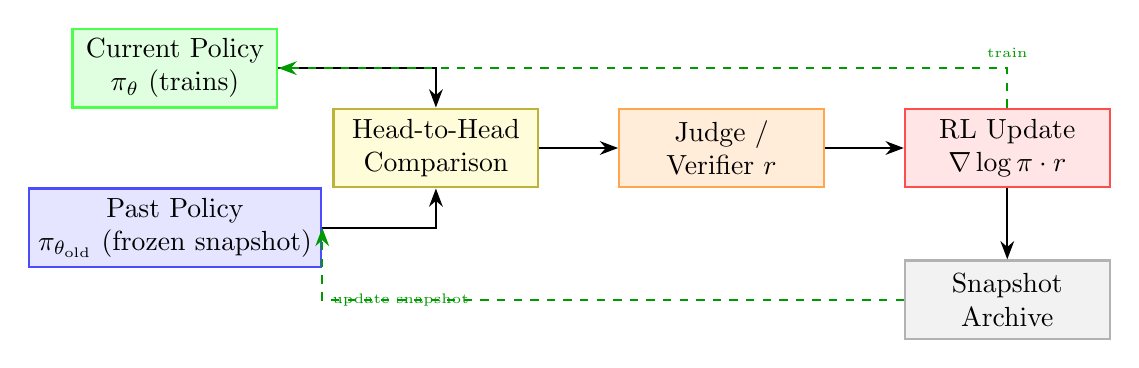
\begin{tikzpicture}[node distance=0.7cm and 1.0cm]
  \node[trnblk] (cur) {Current Policy\\$\pi_\theta$ (trains)};
  \node[frzblk, below=1.0cm of cur] (old) {Past Policy\\$\pi_{\theta_{\text{old}}}$ (frozen snapshot)};
  \node[datblk, right=2.0cm of $(cur)!0.5!(old)$] (game) {Head-to-Head\\Comparison};
  \node[orangeblk, right=of game] (judge) {Judge /\\Verifier $r$};
  \node[lossblk, right=of judge] (rl) {RL Update\\$\nabla\log\pi \cdot r$};
  \node[grayblk, below=0.9cm of rl] (snap) {Snapshot\\Archive};

  \draw[arr] (cur.east) -| (game.north);
  \draw[arr] (old.east) -| (game.south);
  \draw[arr] (game)--(judge);
  \draw[arr] (judge)--(rl);
  \draw[arr] (rl.south)--(snap.north);
  \draw[arr,dashed,green!60!black] (snap.west) -| (old.east) node[midway,right,font=\tiny]{update snapshot};
  \draw[arr,dashed,green!60!black] (rl.north) |- (cur.east) node[midway,above,font=\tiny]{train};
\end{tikzpicture}
\caption{Self-Play RL: current policy competes against a frozen past snapshot; win/loss drives RL updates.}
\end{figure}

\subsection{State Transition Table}
\begin{table}[h]\centering
\begin{tabular}{lll}\toprule
\textbf{Property} & \textbf{Before} & \textbf{After}\\\midrule
Opponent & None / static & Evolving past self\\
Difficulty curriculum & Fixed & Auto-scaling\\
Reward source & External judge & Comparative win/loss\\
Policy snapshot archive & N/A & Maintained\\
Capability ceiling & Fixed by data & Self-determined\\\bottomrule
\end{tabular}
\caption{State properties before and after Self-Play RL setup.}
\end{table}

\newpage
%% ------------------------------------------------------------
\section{Monte Carlo Tree Search RL (MCTS-RL)}

\subsection{Mathematical Foundation}
MCTS-RL builds a reasoning tree by alternating between \emph{selection} (UCT formula), \emph{expansion}, \emph{rollout}, and \emph{backpropagation}. The UCT score for node $n$:
\begin{equation}
  \text{UCT}(n) = \frac{W(n)}{N(n)} + c\sqrt{\frac{\ln N(\text{parent}(n))}{N(n)}}
\end{equation}
where $W(n)$ is total rollout reward and $N(n)$ is visit count. The policy is improved by training on trajectories weighted by MCTS visit counts:
\begin{equation}
  \pi_\theta \leftarrow \pi_\theta + \eta\,\mathbb{E}\bigl[\text{MCTS visits}(a|s) \cdot \nabla_\theta\log\pi_\theta(a|s)\bigr]
\end{equation}

\subsection{Architecture Flow Diagram}

\begin{figure}[h]
\centering
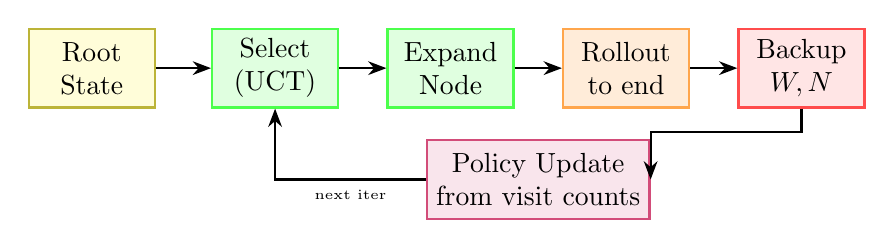
\begin{tikzpicture}[node distance=0.5cm and 0.9cm]
  \node[datblk,minimum width=1.6cm] (root) {Root\\State};
  \node[trnblk, right=0.7cm of root,minimum width=1.6cm] (sel) {Select\\(UCT)};
  \node[trnblk, right=0.6cm of sel,minimum width=1.6cm] (exp) {Expand\\Node};
  \node[orangeblk, right=0.6cm of exp,minimum width=1.6cm] (roll) {Rollout\\to end};
  \node[lossblk, right=0.6cm of roll,minimum width=1.6cm] (back) {Backup\\$W, N$};
  \node[mrgblk, below=0.9cm of $(sel)!0.5!(back)$] (pol) {Policy Update\\from visit counts};

  \draw[arr] (root)--(sel);
  \draw[arr] (sel)--(exp);
  \draw[arr] (exp)--(roll);
  \draw[arr] (roll)--(back);
  \draw[arr] (back.south) -- ++(0,-0.3) -| (pol.east);
  \draw[arr] (pol.west) -| (sel.south) node[near start,below,font=\tiny]{next iter};
\end{tikzpicture}
\caption{MCTS-RL: select (UCT), expand, rollout, backpropagate; visit counts guide policy improvement.}
\end{figure}

\subsection{State Transition Table}
\begin{table}[h]\centering
\begin{tabular}{lll}\toprule
\textbf{Property} & \textbf{Before} & \textbf{After}\\\midrule
Search strategy & Greedy / beam & Tree search (UCT)\\
State value estimate & None & $W(n)/N(n)$ from rollouts\\
Planning horizon & Local & Multi-step look-ahead\\
Compute per query & Inference only & Inference + tree expansion\\
Policy quality & Single-pass & Iteratively refined\\\bottomrule
\end{tabular}
\caption{State properties before and after MCTS-RL integration.}
\end{table}

\newpage
%% ------------------------------------------------------------
\section{Search-Augmented RL (Search-RL)}

\subsection{Mathematical Foundation}
Search-RL augments the reasoning process with an explicit search over candidate next steps. At each step $t$, the policy generates $B$ candidates $\{s_t^{(1)},\ldots,s_t^{(B)}\}$, a verifier scores them, and the best is selected:
\begin{equation}
  s_t^* = \arg\max_{b} V(x, s_{1:t-1}, s_t^{(b)})
\end{equation}
Training uses the full selected trajectory as RL experience:
\begin{equation}
  \mathcal{L}_{\text{SearchRL}} = -\sum_t \mathbb{1}[\mathcal{V}(x,y) = 1]\log\pi_\theta(s_t^* \mid x, s_{1:t-1})
\end{equation}

\subsection{Architecture Flow Diagram}

\begin{figure}[h]
\centering
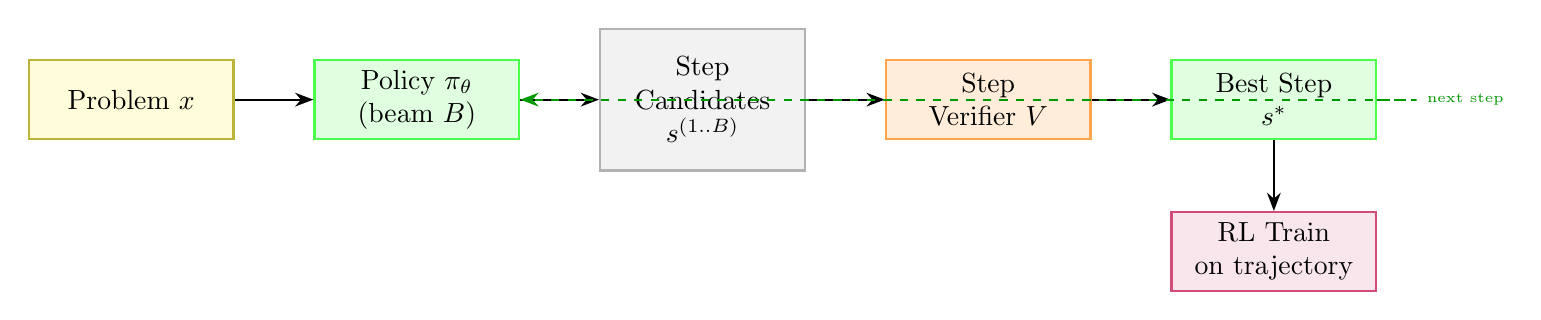
\begin{tikzpicture}[node distance=0.6cm and 1.0cm]
  \node[datblk] (x) {Problem $x$};
  \node[trnblk, right=of x] (pol) {Policy $\pi_\theta$\\(beam $B$)};
  \node[grayblk, right=of pol, minimum height=1.8cm] (cands) {Step\\Candidates\\$s^{(1..B)}$};
  \node[orangeblk, right=of cands] (ver) {Step\\Verifier $V$};
  \node[trnblk, right=of ver] (best) {Best Step\\$s^*$};
  \node[mrgblk, below=0.9cm of best] (train) {RL Train\\on trajectory};

  \draw[arr] (x)--(pol);
  \draw[arr] (pol)--(cands);
  \draw[arr] (cands)--(ver);
  \draw[arr] (ver)--(best);
  \draw[arr] (best.south)--(train.north);
  \draw[arr,dashed,green!60!black] (best.east) -- ++(0.5,0) |- (pol.east) node[midway,right,font=\tiny]{next step};
\end{tikzpicture}
\caption{Search-RL: at each step, beam search generates candidates; verifier selects best; policy trained on trajectory.}
\end{figure}

\subsection{State Transition Table}
\begin{table}[h]\centering
\begin{tabular}{lll}\toprule
\textbf{Property} & \textbf{Before} & \textbf{After}\\\midrule
Step selection & Greedy / top-1 & Verifier-guided beam search\\
Search breadth & 1 & $B$ candidates per step\\
Verifier & None & Step-level verifier $V$\\
Training signal & Outcome reward & Step-selected trajectory\\
Error recovery & None & Search can backtrack\\\bottomrule
\end{tabular}
\caption{State properties before and after Search-RL.}
\end{table}

\newpage
%% ------------------------------------------------------------
\section{Tree-of-Thought Training}

\subsection{Mathematical Foundation}
Tree-of-Thought (ToT) Training teaches the model to generate, evaluate, and prune multiple reasoning branches. The model is trained on annotated trees where each branch $b_i$ has a quality score $q_i \in [0,1]$. The training objective rewards correct branches and penalises dead-ends:
\begin{equation}
  \mathcal{L}_{\text{ToT}} = -\sum_i q_i \sum_t \log P_\theta(b_{i,t} \mid x, b_{i,<t}) + (1-q_i)\sum_t \log(1 - P_\theta(b_{i,t} \mid x, b_{i,<t}))
\end{equation}
A separate scoring model $s_\phi(x, b_i)$ is trained to evaluate intermediate thought nodes and guide beam search at inference.

\subsection{Architecture Flow Diagram}

\begin{figure}[h]
\centering
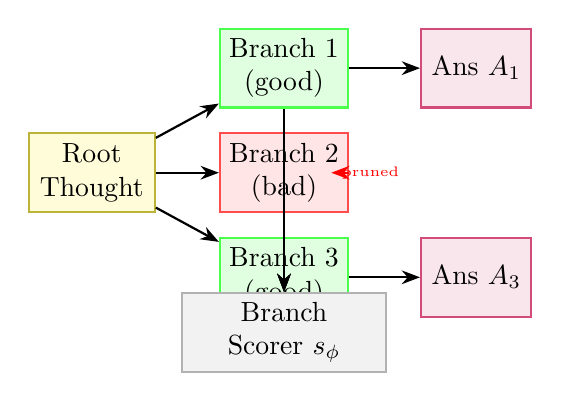
\begin{tikzpicture}[node distance=0.5cm and 0.8cm]
  \node[datblk,minimum width=1.6cm] (root) {Root\\Thought};
  \node[trnblk,minimum width=1.4cm, above right=0.3cm and 0.8cm of root] (b1) {Branch 1\\(good)};
  \node[lossblk,minimum width=1.4cm, right=0.3cm and 0.8cm of root] (b2) {Branch 2\\(bad)};
  \node[trnblk,minimum width=1.4cm, below right=0.3cm and 0.8cm of root] (b3) {Branch 3\\(good)};
  \node[mrgblk,minimum width=1.4cm, right=0.9cm of b1] (ans1) {Ans $A_1$};
  \node[mrgblk,minimum width=1.4cm, right=0.9cm of b3] (ans3) {Ans $A_3$};
  \node[grayblk, below=1.0cm of b2] (score) {Branch\\Scorer $s_\phi$};

  \draw[arr] (root)--(b1);
  \draw[arr] (root)--(b2);
  \draw[arr] (root)--(b3);
  \draw[arr] (b1)--(ans1);
  \draw[arr] (b3)--(ans3);
  \draw[arr,red,dashed] (b2) -- ++(0.6,0) node[right,font=\tiny,red]{pruned};
  \draw[arr] (b1.south) -| (score.north);
  \draw[arr] (b2.south) -- (score.north);
  \draw[arr] (b3.north) -| (score.north);
\end{tikzpicture}
\caption{ToT Training: good branches lead to answers; bad branches are pruned; scorer trained to evaluate all.}
\end{figure}

\subsection{State Transition Table}
\begin{table}[h]\centering
\begin{tabular}{lll}\toprule
\textbf{Property} & \textbf{Before} & \textbf{After}\\\midrule
Reasoning structure & Linear chain & Branching tree\\
Dead-end handling & None & Explicit pruning\\
Branch evaluator & None & Trained $s_\phi$\\
Search at inference & Linear & Guided tree beam\\
Complex planning & Weak & Strong\\\bottomrule
\end{tabular}
\caption{State properties before and after Tree-of-Thought Training.}
\end{table}

\newpage
%% ------------------------------------------------------------
\section{Self-Consistency Training}

\subsection{Mathematical Foundation}
Self-Consistency Training generates $K$ independent reasoning paths and uses majority voting to determine the correct answer. The model is then trained to increase probability of the majority-vote answer $y^*$:
\begin{equation}
  y^* = \arg\max_{y} \sum_{k=1}^K \mathbf{1}[\text{answer}(y^{(k)}) = y],\quad y^{(k)} \sim \pi_\theta(\cdot|x)
\end{equation}
\begin{equation}
  \mathcal{L}_{\text{SC}} = -\sum_{\{k:\,\text{answer}(y^{(k)})=y^*\}} \sum_t \log P_\theta(y^{(k)}_t \mid x, y^{(k)}_{<t})
\end{equation}
Paths that agree with the majority vote are reinforced; minority paths are not trained on (or penalised).

\subsection{Architecture Flow Diagram}

\begin{figure}[h]
\centering
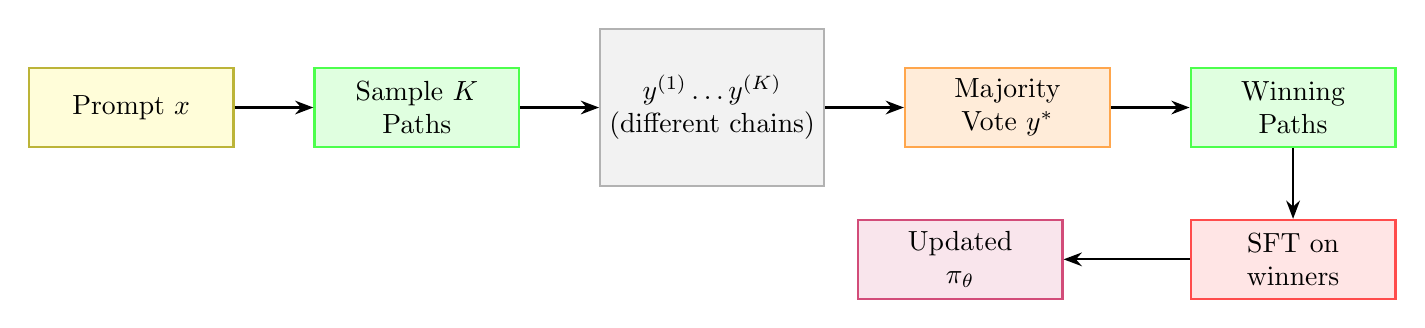
\begin{tikzpicture}[node distance=0.6cm and 1.0cm]
  \node[datblk] (x) {Prompt $x$};
  \node[trnblk, right=of x] (pol) {Sample $K$\\Paths};
  \node[grayblk, right=of pol, minimum height=2.0cm] (paths) {$y^{(1)}\ldots y^{(K)}$\\(different chains)};
  \node[orangeblk, right=of paths] (vote) {Majority\\Vote $y^*$};
  \node[trnblk, right=of vote] (winners) {Winning\\Paths};
  \node[lossblk, below=0.9cm of winners] (sft) {SFT on\\winners};
  \node[mrgblk, left=1.6cm of sft] (out) {Updated\\$\pi_\theta$};

  \draw[arr] (x)--(pol);
  \draw[arr] (pol)--(paths);
  \draw[arr] (paths)--(vote);
  \draw[arr] (vote)--(winners);
  \draw[arr] (winners)--(sft);
  \draw[arr] (sft)--(out);
\end{tikzpicture}
\caption{Self-Consistency Training: majority-vote over $K$ paths identifies winning chains; model trained on those.}
\end{figure}

\subsection{State Transition Table}
\begin{table}[h]\centering
\begin{tabular}{lll}\toprule
\textbf{Property} & \textbf{Before} & \textbf{After}\\\midrule
Inference mode & Single greedy & $K$ diverse samples\\
Answer selection & Argmax & Majority vote\\
Training target & All completions & Majority-consistent paths only\\
Accuracy ceiling & Limited by single pass & Higher (ensemble effect)\\
Compute cost & $1\times$ & $K\times$ at sampling time\\\bottomrule
\end{tabular}
\caption{State properties before and after Self-Consistency Training.}
\end{table}

\newpage
%% ============================================================
\part{Reward Modeling}
%% ============================================================

\section{Reward Model (RM)}

\subsection{Mathematical Foundation}
A Reward Model takes a prompt $x$ and a completion $y$ and outputs a scalar preference score. It is trained on human-ranked pairs $(y_w \succ y_l)$ via the Bradley-Terry log-likelihood:
\begin{equation}
  \mathcal{L}_{\text{RM}} = -\mathbb{E}_{(x,y_w,y_l)}\bigl[\log\sigma(r_\phi(x,y_w) - r_\phi(x,y_l))\bigr]
\end{equation}
The RM is typically initialised from a fine-tuned LLM with the final token's hidden state projected to a scalar via a linear head $W_r \in \mathbb{R}^{d \times 1}$:
\begin{equation}
  r_\phi(x,y) = W_r^\top h_{\text{last}}(x,y)
\end{equation}

\subsection{Architecture Flow Diagram}

\begin{figure}[h]
\centering
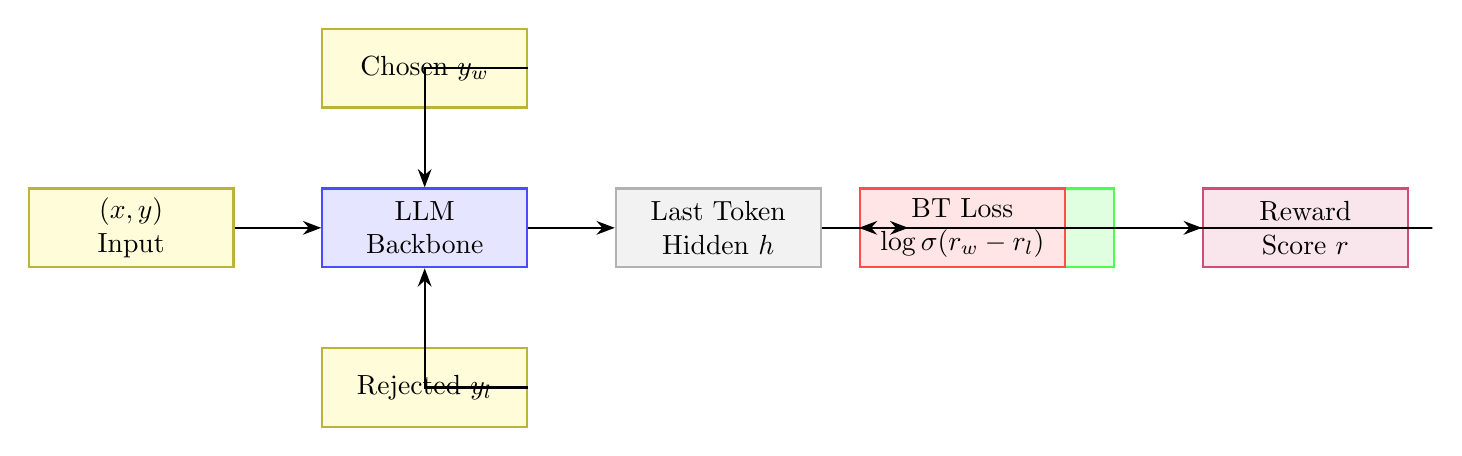
\begin{tikzpicture}[node distance=0.7cm and 1.1cm]
  \node[datblk] (inp) {$(x, y)$\\Input};
  \node[frzblk, right=of inp] (backbone) {LLM\\Backbone};
  \node[grayblk, right=of backbone] (last) {Last Token\\Hidden $h$};
  \node[trnblk, right=of last] (head) {Scalar\\Head $W_r$};
  \node[mrgblk, right=of head] (score) {Reward\\Score $r$};

  \node[datblk, above=1.0cm of backbone] (yw) {Chosen $y_w$};
  \node[datblk, below=1.0cm of backbone] (yl) {Rejected $y_l$};
  \node[lossblk, right=4.2cm of backbone] (loss) {BT Loss\\$\log\sigma(r_w - r_l)$};

  \draw[arr] (inp)--(backbone);
  \draw[arr] (backbone)--(last);
  \draw[arr] (last)--(head);
  \draw[arr] (head)--(score);
  \draw[arr] (yw.east) -| (backbone.north);
  \draw[arr] (yl.east) -| (backbone.south);
  \draw[arr] (score.east) -- ++(0.3,0) |- (loss.west);
\end{tikzpicture}
\caption{Reward Model: LLM backbone maps $(x,y)$ pair to scalar via linear head; trained on chosen/rejected pairs.}
\end{figure}

\subsection{State Transition Table}
\begin{table}[h]\centering
\begin{tabular}{lll}\toprule
\textbf{Property} & \textbf{Before} & \textbf{After}\\\midrule
Output type & Token distribution & Scalar reward\\
Final layer & LM head & Scalar head $W_r$\\
Training data & Text completions & $(x, y_w, y_l)$ preference pairs\\
Loss function & Cross-entropy & Bradley-Terry log-likelihood\\
Usage & Language generation & RLHF reward signal\\\bottomrule
\end{tabular}
\caption{State properties before and after reward model training.}
\end{table}

\newpage
%% ------------------------------------------------------------
\section{Process Reward Model (PRM)}

\subsection{Mathematical Foundation}
A PRM assigns a reward to each intermediate reasoning step $s_t$ rather than to the final answer alone. Given a solution prefix $(s_1,\ldots,s_t)$, the PRM outputs a binary step quality $q_t \in \{0,1\}$:
\begin{equation}
  r_{\text{PRM}}(x, s_{1:T}) = \prod_{t=1}^T r_t,\quad r_t = P_\phi(q_t = 1 \mid x, s_{1:t})
\end{equation}
The PRM is trained on step-level human labels with binary cross-entropy:
\begin{equation}
  \mathcal{L}_{\text{PRM}} = -\sum_t \bigl[q_t \log r_t + (1-q_t)\log(1-r_t)\bigr]
\end{equation}

\subsection{Architecture Flow Diagram}

\begin{figure}[h]
\centering
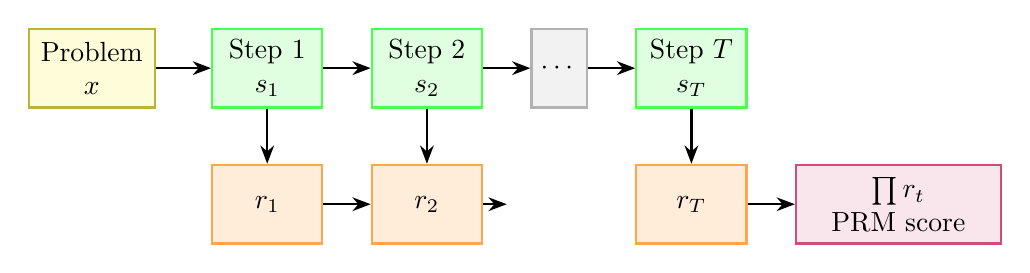
\begin{tikzpicture}[node distance=0.5cm and 0.8cm]
  \node[datblk,minimum width=1.6cm] (x) {Problem\\$x$};
  \node[trnblk,minimum width=1.4cm, right=0.7cm of x] (s1) {Step 1\\$s_1$};
  \node[trnblk,minimum width=1.4cm, right=0.6cm of s1] (s2) {Step 2\\$s_2$};
  \node[grayblk,minimum width=0.6cm, right=0.6cm of s2] (dots) {$\cdots$};
  \node[trnblk,minimum width=1.4cm, right=0.6cm of dots] (sT) {Step $T$\\$s_T$};

  \node[orangeblk,minimum width=1.4cm, below=0.7cm of s1] (r1) {$r_1$};
  \node[orangeblk,minimum width=1.4cm, below=0.7cm of s2] (r2) {$r_2$};
  \node[orangeblk,minimum width=1.4cm, below=0.7cm of sT] (rT) {$r_T$};
  \node[mrgblk, right=0.6cm of rT] (prod) {$\prod r_t$\\PRM score};

  \foreach \s/\r in {s1/r1, s2/r2, sT/rT}
    \draw[arr] (\s)--(\r);
  \draw[arr] (r1.east) -- (r2.west);
  \draw[arr] (r2.east) -- ++(0.3,0);
  \draw[arr] (rT)--(prod);
  \foreach \a/\b in {x/s1, s1/s2, s2/dots, dots/sT}
    \draw[arr] (\a)--(\b);
\end{tikzpicture}
\caption{PRM: each reasoning step independently scored; product of step scores gives overall process reward.}
\end{figure}

\subsection{State Transition Table}
\begin{table}[h]\centering
\begin{tabular}{lll}\toprule
\textbf{Property} & \textbf{Before (RM)} & \textbf{After (PRM)}\\\midrule
Reward granularity & Final answer only & Per-step\\
Error localisation & None & Identifies failing step\\
Label annotation & Answer-level & Step-level (expensive)\\
Reward signal density & Sparse (1 per traj.) & Dense ($T$ per traj.)\\
Training on correct solutions & Required & Not required\\\bottomrule
\end{tabular}
\caption{State properties comparing RM and PRM.}
\end{table}

\newpage
%% ------------------------------------------------------------
\section{Outcome Reward Model (ORM)}

\subsection{Mathematical Foundation}
An ORM judges only the \emph{correctness of the final answer} $y_{\text{ans}}$, ignoring intermediate steps. For verifiable tasks (math, code), correctness can be checked automatically:
\begin{equation}
  r_{\text{ORM}}(x, y) = \mathbf{1}[\text{verify}(y_{\text{ans}}, y^*_{\text{gold}})]
\end{equation}
For open-ended tasks, the ORM is a learned binary classifier trained on (correct, incorrect) outcome labels:
\begin{equation}
  \mathcal{L}_{\text{ORM}} = -\bigl[c\log P_\phi(y) + (1-c)\log(1-P_\phi(y))\bigr],\quad c \in \{0,1\}
\end{equation}

\subsection{Architecture Flow Diagram}

\begin{figure}[h]
\centering
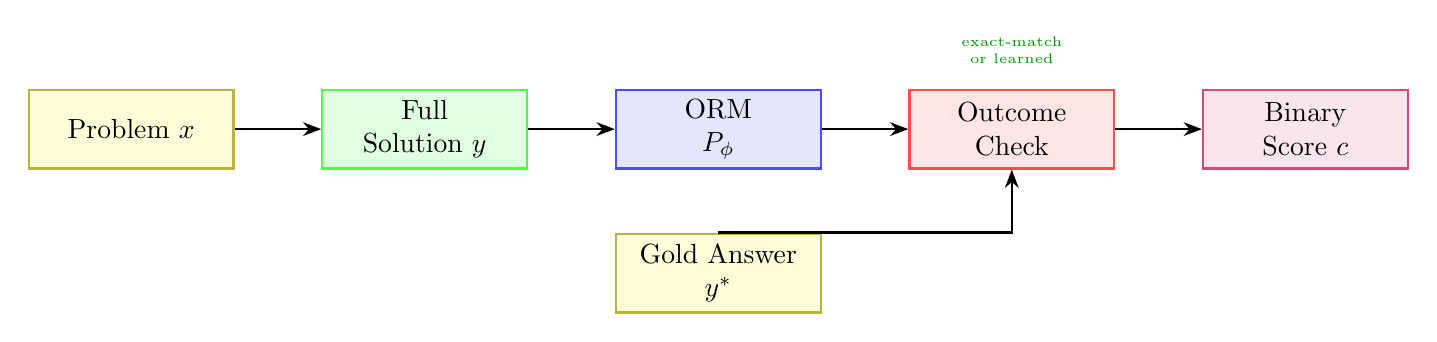
\begin{tikzpicture}[node distance=0.7cm and 1.1cm]
  \node[datblk] (x) {Problem $x$};
  \node[trnblk, right=of x] (sol) {Full\\Solution $y$};
  \node[frzblk, right=of sol] (lm) {ORM\\$P_\phi$};
  \node[lossblk, right=of lm] (check) {Outcome\\Check};
  \node[mrgblk, right=of check] (score) {Binary\\Score $c$};

  \node[datblk,below=0.8cm of lm] (gold) {Gold Answer\\$y^*$};

  \draw[arr] (x)--(sol);
  \draw[arr] (sol)--(lm);
  \draw[arr] (lm)--(check);
  \draw[arr] (gold.north)-|(check.south);
  \draw[arr] (check)--(score);

  \node[font=\tiny,green!60!black,align=center,above=0.2cm of check] {exact-match\\or learned};
\end{tikzpicture}
\caption{ORM: scores the final answer against gold; can be rule-based (exact-match) or learned classifier.}
\end{figure}

\subsection{State Transition Table}
\begin{table}[h]\centering
\begin{tabular}{lll}\toprule
\textbf{Property} & \textbf{Before} & \textbf{After}\\\midrule
Reward scope & N/A & Final answer only\\
Intermediate credit & None & None\\
Annotation cost & N/A & Low (binary label)\\
Verifiable tasks & Manual check & Automatic (rule-based)\\
Open-ended tasks & None & Learned classifier\\\bottomrule
\end{tabular}
\caption{State properties before and after ORM setup.}
\end{table}

\newpage
%% ------------------------------------------------------------
\section{Verifier Model}

\subsection{Mathematical Foundation}
A Verifier Model is a binary classifier that determines whether a candidate solution is correct. Unlike an ORM that outputs a probability, verifiers typically use a hard decision rule learned from (correct, incorrect) solution pairs:
\begin{equation}
  \hat{v}(x, y) = \mathbf{1}\bigl[P_\phi(\text{correct} \mid x, y) \geq \tau\bigr]
\end{equation}
Verifiers are used in test-time search (Best-of-N) and training-time filtering (RFT). The decision threshold $\tau$ trades off precision and recall on the verification task:
\begin{equation}
  \mathcal{L}_{\text{ver}} = -\bigl[v\log P_\phi + (1-v)\log(1-P_\phi)\bigr],\quad v \in \{0,1\}
\end{equation}

\subsection{Architecture Flow Diagram}

\begin{figure}[h]
\centering
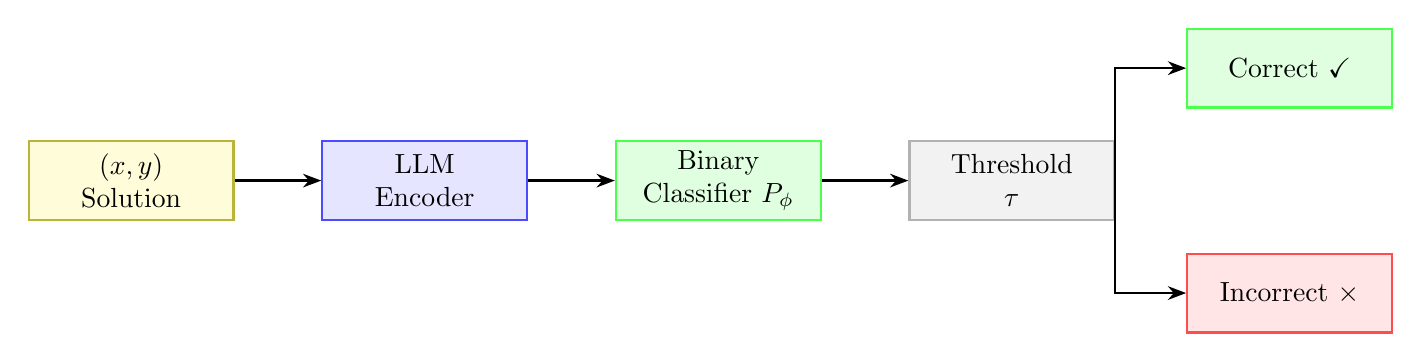
\begin{tikzpicture}[node distance=0.7cm and 1.1cm]
  \node[datblk] (x) {$(x, y)$\\Solution};
  \node[frzblk, right=of x] (enc) {LLM\\Encoder};
  \node[trnblk, right=of enc] (cls) {Binary\\Classifier $P_\phi$};
  \node[grayblk, right=of cls] (thr) {Threshold\\$\tau$};
  \node[trnblk, above right=0.4cm and 0.9cm of thr] (yes) {Correct $\checkmark$};
  \node[lossblk, below right=0.4cm and 0.9cm of thr] (no) {Incorrect $\times$};

  \draw[arr] (x)--(enc);
  \draw[arr] (enc)--(cls);
  \draw[arr] (cls)--(thr);
  \draw[arr] (thr.east) |- (yes.west);
  \draw[arr] (thr.east) |- (no.west);
\end{tikzpicture}
\caption{Verifier Model: encodes solution, classifies as correct/incorrect via learned threshold.}
\end{figure}

\subsection{State Transition Table}
\begin{table}[h]\centering
\begin{tabular}{lll}\toprule
\textbf{Property} & \textbf{Before} & \textbf{After}\\\midrule
Output & Continuous score & Binary decision\\
Threshold & N/A & Tunable $\tau$\\
Primary use & Ranking & Filtering (accept/reject)\\
Training data & Ranked pairs & Correct/incorrect labels\\
Precision/recall trade-off & N/A & Controlled via $\tau$\\\bottomrule
\end{tabular}
\caption{State properties before and after Verifier Model training.}
\end{table}

\newpage
%% ------------------------------------------------------------
\section{Critic Model}

\subsection{Mathematical Foundation}
A Critic Model generates natural-language \emph{critiques} of candidate outputs and optionally a numerical score. It is trained on (output, critique, revision) triplets. The critique generation loss:
\begin{equation}
  \mathcal{L}_{\text{crit}} = -\sum_t \log P_\phi(c_t \mid x, y, c_{<t})
\end{equation}
where $c$ is the gold critique. Critics enable self-refinement loops: the model generates $y$, the critic evaluates it producing $c$, and the model revises $y \to y'$ conditioned on $(x, y, c)$:
\begin{equation}
  y' \sim P_\theta(\cdot \mid x, y, c)
\end{equation}

\subsection{Architecture Flow Diagram}

\begin{figure}[h]
\centering
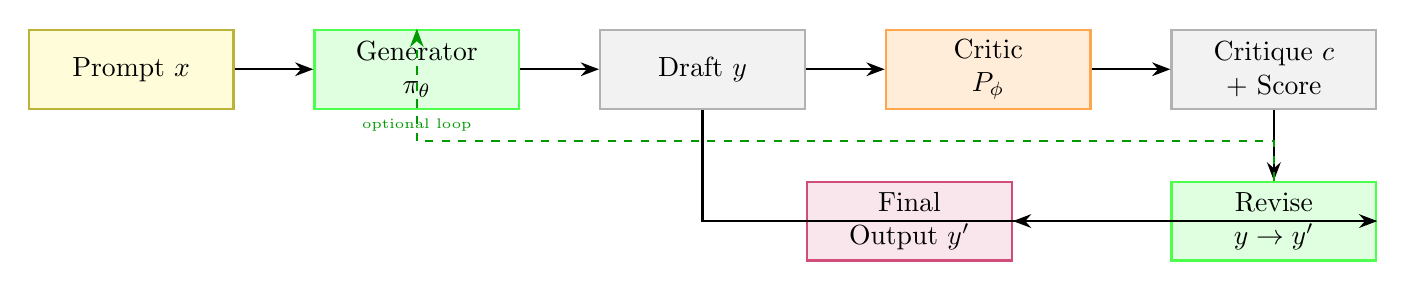
\begin{tikzpicture}[node distance=0.7cm and 1.0cm]
  \node[datblk] (x) {Prompt $x$};
  \node[trnblk, right=of x] (gen) {Generator\\$\pi_\theta$};
  \node[grayblk, right=of gen] (y) {Draft $y$};
  \node[orangeblk, right=of y] (crit) {Critic\\$P_\phi$};
  \node[grayblk, right=of crit] (c) {Critique $c$\\+ Score};
  \node[trnblk, below=0.9cm of c] (rev) {Revise\\$y \to y'$};
  \node[mrgblk, left=2.0cm of rev] (out) {Final\\Output $y'$};

  \draw[arr] (x)--(gen);
  \draw[arr] (gen)--(y);
  \draw[arr] (y)--(crit);
  \draw[arr] (crit)--(c);
  \draw[arr] (c)--(rev);
  \draw[arr] (y.south) |- (rev.east);
  \draw[arr] (rev)--(out);
  \draw[arr,dashed,green!60!black] (rev.north) -- ++(0,0.5) -| (gen.north) node[midway,above,font=\tiny]{optional loop};
\end{tikzpicture}
\caption{Critic Model: generates natural-language critique of a draft; generator revises using the critique.}
\end{figure}

\subsection{State Transition Table}
\begin{table}[h]\centering
\begin{tabular}{lll}\toprule
\textbf{Property} & \textbf{Before} & \textbf{After}\\\midrule
Feedback type & Scalar reward & Natural-language critique\\
Interpretability & Low (scalar) & High (textual feedback)\\
Revision loop & Not applicable & Generator refines on critique\\
Training data & Preference pairs & (output, critique, revision) triplets\\
Use case & RM scoring & Self-refinement / RLHF\\\bottomrule
\end{tabular}
\caption{State properties before and after Critic Model training.}
\end{table}

\end{document}
